\documentclass[12pt,a4paper,twoside]{article}
\usepackage{labor}
\begin{document}

%fill for cover and header creation
\newcommand\laboratorynumber{2}
\title{Phase/Leistung}
\newcommand\supervisor{Ditlbacher, Harald}
\newcommand\groupnumber{42}

\newcommand\participantonelastname{Eisner}
\newcommand\participantonefirstname{Nico}
\newcommand\participantoneid{12214121}
\newcommand\participanttwolastname{Waldl}
\newcommand\participanttwofirstname{Philip}
\newcommand\participanttwoid{12214120}
\author{\participantonelastname \ \& \participanttwolastname}

\newcommand\degreeid{UB 033 678}
\newcommand\semester{23WS}
\date{15.12.2023}

%select correct course title
%\newcommand\coursetitle{Einführung in die \\ physikalischen Messmethoden}
%\newcommand\coursetitle{Laborübungen 1: \\ Mechanik und Wärme}
\newcommand\coursetitle{Laborübungen 2: \\ Elektrizität, Magnetismus, Optik}
%\newcommand\coursetitle{Fortgeschrittenen Praktikum 1: \\ Technische Physik}
%\newcommand\coursetitle{Fortgeschrittenen Praktikum 2: \\ Allgemeine Physik}

%\begin{titlepage}
   \begin{center}
       \begin{figure}[H]
            \begin{minipage}[h]{30mm}
                \centerline{
\includegraphics[height=15mm]{cover_nudes/tugraz.png}}
            \end{minipage}
            \hfill
            \begin{minipage}[h]{30mm}
                \centerline{
\includegraphics[height=15mm]{cover_nudes/nawi_graz.png}}
            \end{minipage}
            \hfill
            \begin{minipage}[h]{30mm}
                \centerline{
\includegraphics[height=15mm]{cover_nudes/uni-graz.png}}
            \end{minipage}
        \end{figure}
        
        \large{\emph{Institut für Experimentalphysik der Technischen Universität Graz \\
        \& Institut für Physik der Universität Graz}} \\
        \vspace{5mm}
        
        {\Huge \textbf{\coursetitle}}
        \vspace{5mm}
        
        {\huge \laboratorynumber: \thetitle}
    \end{center}
    
    \vfill
    
    \begin{table}[H]
        \LARGE
        \centering
        \begin{tabular}{r l}
            Betreuer:       & \supervisor \\
            Gruppennummer:  & \groupnumber \\
            \\
            Name:           & \participantonelastname, \participantonefirstname \\
            Matrikelnummer: & \participantoneid \\
            Name:           & \participanttwolastname, \participanttwofirstname \\
            Matrikelnummer: & \participanttwoid \\
            \\
            Kennzahl:       & \degreeid \\
            Datum:          & \semester \ | \thedate
        \end{tabular}
    \end{table}
    \vspace{4cm}
\end{titlepage}
\clearpage
\setcounter{page}{1}

%\maketitle %short title alternative

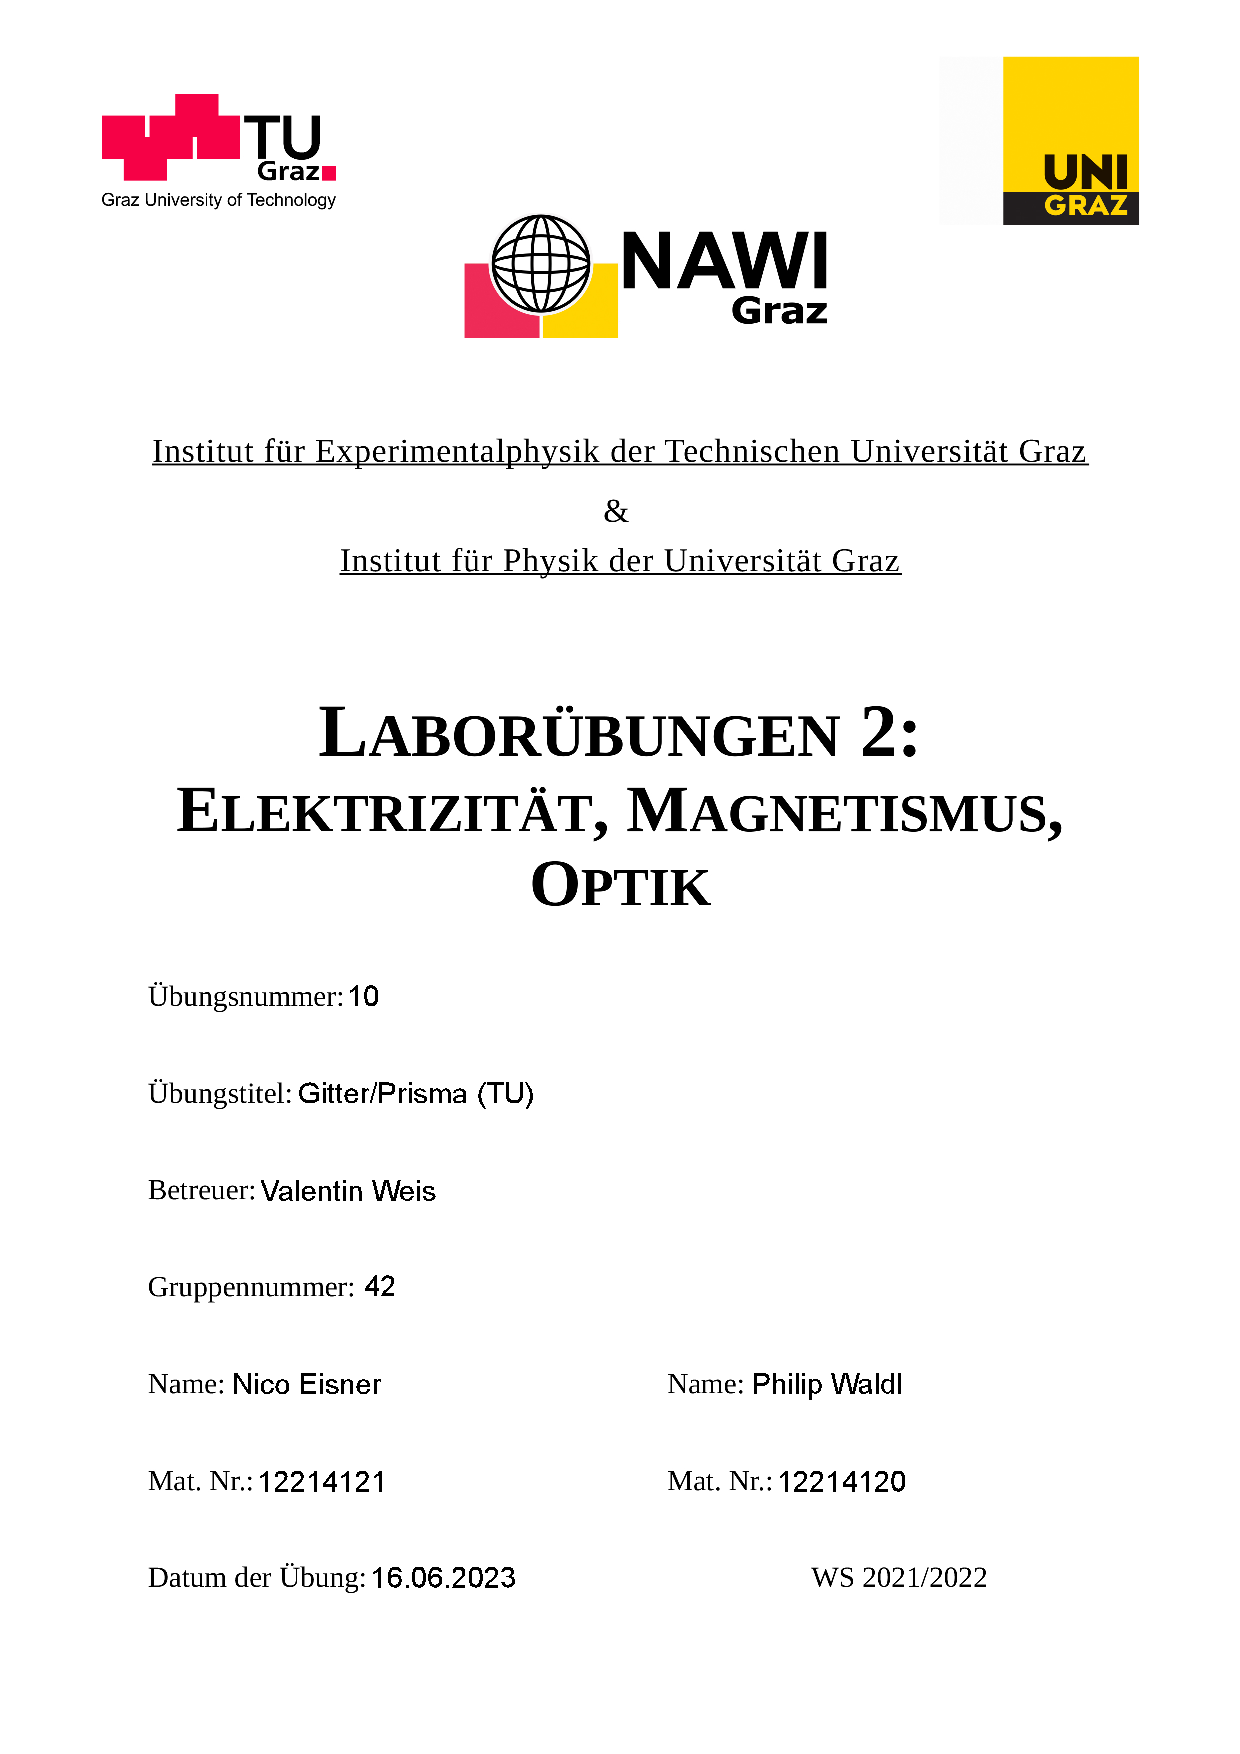
\includepdf[pages={1}]{../Deckblätter/Deckblatt_Gitter.pdf}

\tableofcontents
\newpage

\section{Aufgabenstellung} %jo beschreibn wos gmocht host ------------------------------

Beim Versuch Phase Leistung dreht sich alles um die Phasenlage von Strom und Spannung bzw. die elektrische Leistung.
Diese Größen sollen in verschiednenen Schaltungen praktisch ermittelt und ausgewertet werden. Die genaue Aufgabenstellung hierfür sieht wie folgt aus:

\begin{itemize}
    \item Untersuchung der Anzeige von unterschiedlichen Spannungsmessinstrumenten bei verschiednenen Spannungsformen
    \item Amlitudengang von verschiedenen Spannungsmessinstrumenten
    \item Phasenlage $\phi_C$ von Strom/Spannung an einem Kondensator
    \item Phasenlage $\phi_L$ von Strom/Spannung an einer Spule
    \item Elektrische Leistung $P_{RC}$ in einer RC-Schaltung
    \item Elektrische Leistung $P_{RL}$ in einer RL-Schaltung
    \item Untersuchungen zur Blindleistungskompensation
\end{itemize}

\noindent
Alle Informationen und Methodiken wurden uns von der Technischen Universität bereitgestellt \cite{teachcenter2}. 



\section{Voraussetzungen \& Grundlagen} %Grundlagen erklären, Formeln mit erklärung

\subsection{Kenngrößen}

Zu Beginn der Grundlagen ist es wichtig, einige Größen zu definieren.

\begin{table}[H]
    \centering
    \caption{Definitionen \cite{teachcenter2}}
    \label{tab:definitionen}
    \begin{tabular}{| l | l |}
        \hline
        Scheitelwert & Der größte Betrag der Augenblickswerte eines Wechselsignals. \\
        Effektivwert & Wert einer Gleichspannung / eines Gleichstromes, die / der an einem ohmschen \\
         & Widerstand im zeitlichen Mittel die gleiche Leistung wie die entsprechende \\
         & Wechselspannung / der entsprechende Wechselstrom. \\
        Gleichrichtwert & Mittelwert des Betrages der Spannung / des Stromes. \\
        Formfaktor & Verhältnis von Effektivwert zu Gleichrichtwert. \\
        Scheitelfaktor & Verhältnis von Scheitelwert zu Effektivwert. \\
        \hline
    \end{tabular}
\end{table}

\subsection{Komplexe Wechselstromtechnik}

Die beliebteste Signalart, welche auch am häufigsten verwendet wird, ist in der Wechselstromtechnik die Sinusspannung. 
Ohm`sche Widerstände verursachen hier keine Phasenverschiebung zwischen Strom und Spannung. Kapazitive- und Induktive Widerstände jedoch führen zu einer positiven bzw. negativen Phasenverschiebung zwischen diesen Größen.
Deshalb müssen in der Wechselstromtechnik Reaktanzen definiert werden, welche auch Blindwiderstände genannt werden. 
Diese hängen von der verwendeten Frequenz und den Kapazitäten bzw. Induktivitäten ab (Formeln in Abteil Wichtige Zusammenhänge).
Diese Reaktanzen bilden im Prinzip das Äquivalent zu den herkörmlichen Widerständen an ohm`schen Verbrauchern.
Weiters können daraus komplexe Impedanzen Z gebildet werden, welche zusätzlich zu den Signalstärken auch die Signalverschiebung beschreiben. 




\subsection{Leistung und Verluste}

Die Leistung, die von einem Stromnetz tatsächlich benötigt wird, wird auch Scheinleistung S [VA] genannt. Diese setzt sich aus dem Produkt der Effektivwerte von Strom I und Spannung U zusammen.
Der Realteil der Scheinleistung stellt dabei die Wirkleistung P, angegeben in Watt, dar. Diese beschreibt die Leistung an den ohm`schen Verbrauchen. Der Imaninärteil wird auch Bindleistung Q [var] genannt und bezeichnet jene Leistung, welche für die ohm`schen Verbraucher keinen Nutzen hat.
Sie kommt durch verschiedene Phänomene zustande, wie z.B. Aufbau von B-Feldern bei Induktion. \newline

\noindent
Um letztere Leistung zu verringen wird auf das Prinzip der Blindleistungskompensation gesetzt. Dabei werden Blindleistungsanteile durch gezieltes hinzufügen von bestimmten Kondensatoren und Spulen möglichst klein gehalten. Dadurch, dass auch jedes kapazitive- und induktive Bauteil einen ohm`schen Innenwiderstand besitzt und somit Verluste aufweist, gibt es in der realen Umgebung keine Blindwiderstände. 



 \subsection{Wichtige Zusammenhänge}

 \begin{equation}
    \label{eq:Phasenversatz}
    \centerline{$\Phi = \frac{360°}{T}*\Delta t = 360° * \Delta t * f$ \\ $\Delta \Phi = \vert \frac{\partial \Phi}{\partial \Delta t} * \Delta \Delta t \vert + \vert \frac{\partial \Phi}{\partial f} * \Delta f \vert $}
\end{equation}

\begin{equation}
    \label{eq:Phasenversatz_Kreise}
    \centerline{$\Phi $ = $arg(U)$ = $\arctan(\frac{U_{C}sin(\phi_C)}{U_R + U_{C}cos(\phi_C)}$) \\ $\Delta \Phi = \vert \frac{\partial \Phi}{\partial U_{C}} * \Delta U_{C} \vert + \vert \frac{\partial \Phi}{\partial U_R} * \Delta U_R \vert + \vert \frac{\partial \Phi}{\partial \phi_C} * \Delta \phi_C \vert$}
\end{equation}

\begin{equation}
    \label{eq:Scheinleistung}
    \centerline{$S $ = UI   \\ $\Delta P = \vert \frac{\partial P}{\partial U} * \Delta Uu \vert + \vert \frac{\partial S}{\partial I} * \Delta I \vert$}
\end{equation}

\begin{equation}
    \label{eq:Wirkleistung}
    \centerline{$P $ = $S*cos(\phi)$  \\ $\Delta P = \vert \frac{\partial P}{\partial S} * \Delta S \vert + \vert \frac{\partial P}{\partial \phi} * \Delta \phi \vert$ }
\end{equation}

\begin{equation}
    \label{eq:Blindleistung}
    \centerline{$Q $ = $S*sin(\phi)$  \\ $\Delta Q = \vert \frac{\partial Q}{\partial S} * \Delta S \vert + \vert \frac{\partial Q}{\partial \phi} * \Delta \phi \vert$}
\end{equation}

\begin{equation}
    \label{eq:ReaktanzenC}
    \centerline{$X_{C}$ = $-\frac{1}{\omega C}$ \\ $\Delta X_{C} = \vert \frac{\partial X_{C}}{\partial C} * \Delta C \vert $}
\end{equation}

\begin{equation}
    \label{eq:ReaktanzenL}
    \centerline{$X_{L}$ = $\omega L$ \\ $\Delta X_{L} = \vert \frac{\partial X_{L}}{\partial L} * \Delta L \vert $} 
\end{equation}



\section{Versuchsanordnung} %mit skizze kurz beschreiben ------------------------------

Wie im Punkt Aufgabenstellung bereits erwähnt, beinhaltet der Versuch mehrere Versuchsaufbauten.

\subsection{Untersuchung der Anzeigen}

Für den ersten Teil wird eine Schaltung mit folgenden Aufbau realisiert:

\begin{figure}[H]
    \centering
    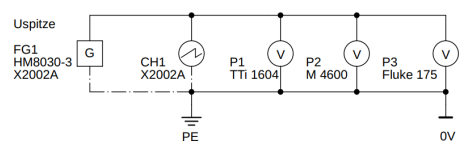
\includegraphics[width=0.4\linewidth]{nudes/Schaltplan1.PNG}
    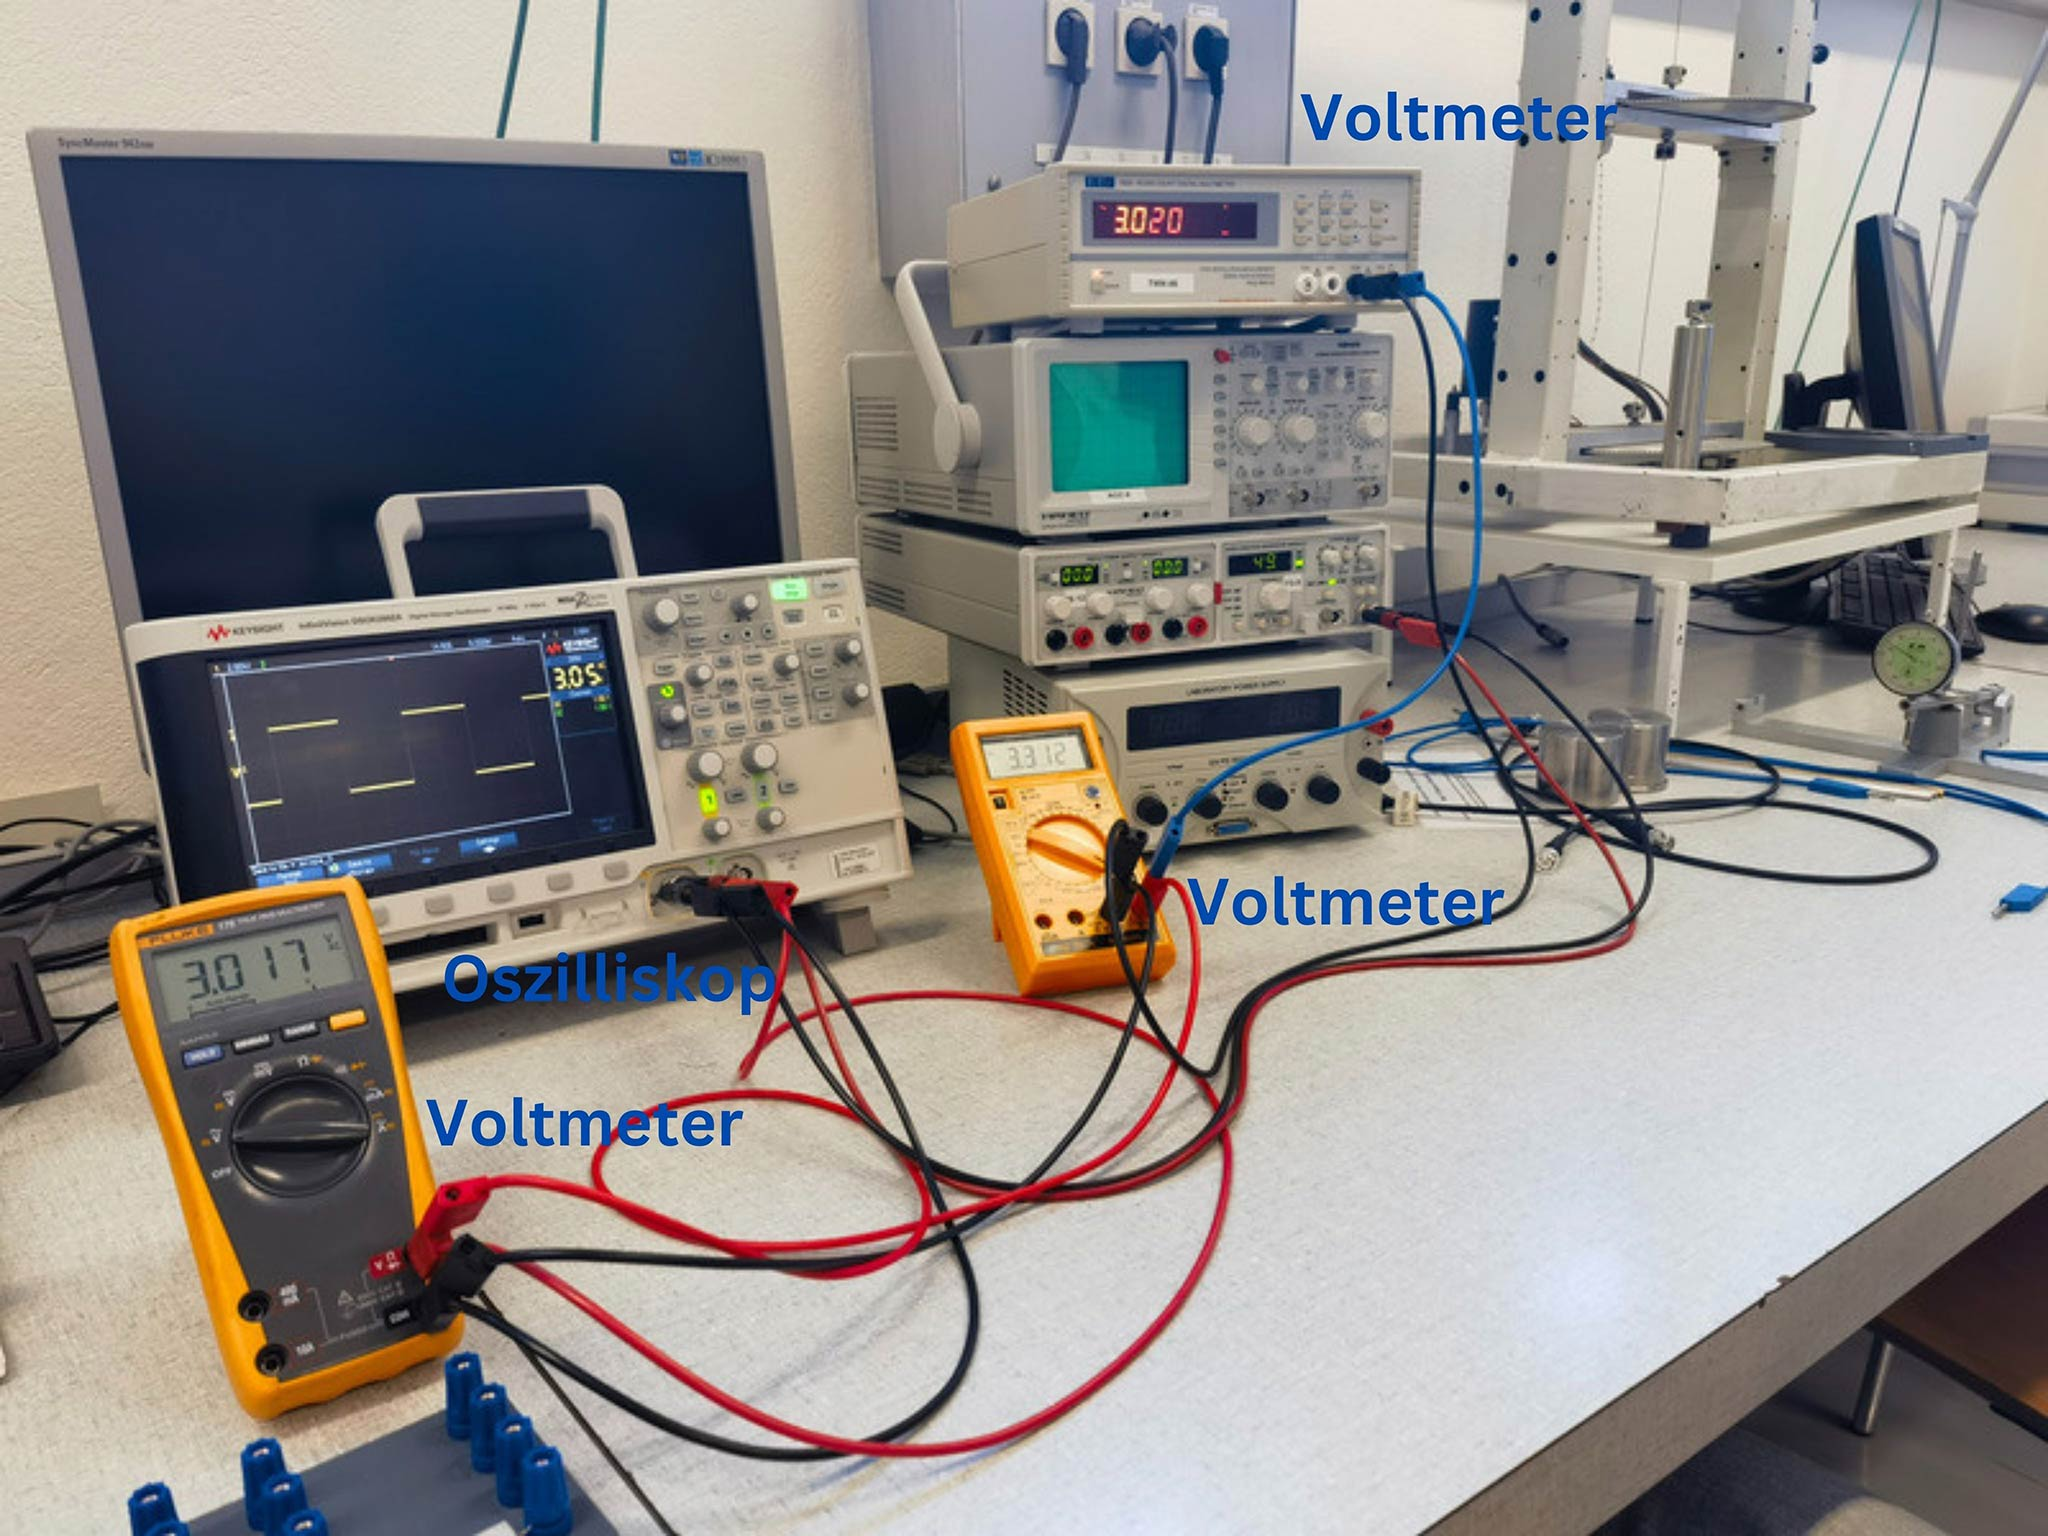
\includegraphics[width=0.4\linewidth]{nudes/PhaseLeistungBilder/Aufbau1,2.jpg}
    \caption{Schaltplan und realer Aufbau zur Untersuchung der Anzeigen}
    \label{fig:Aufbau1}
\end{figure}


\subsection{Amplitudengänge}

Die Amplitudengänge wurden mit der gleichen Schaltung ermittelt:

\begin{figure}[H]
    \centering
    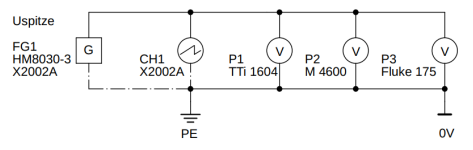
\includegraphics[width=0.4\linewidth]{nudes/Schaltplan2.PNG}
    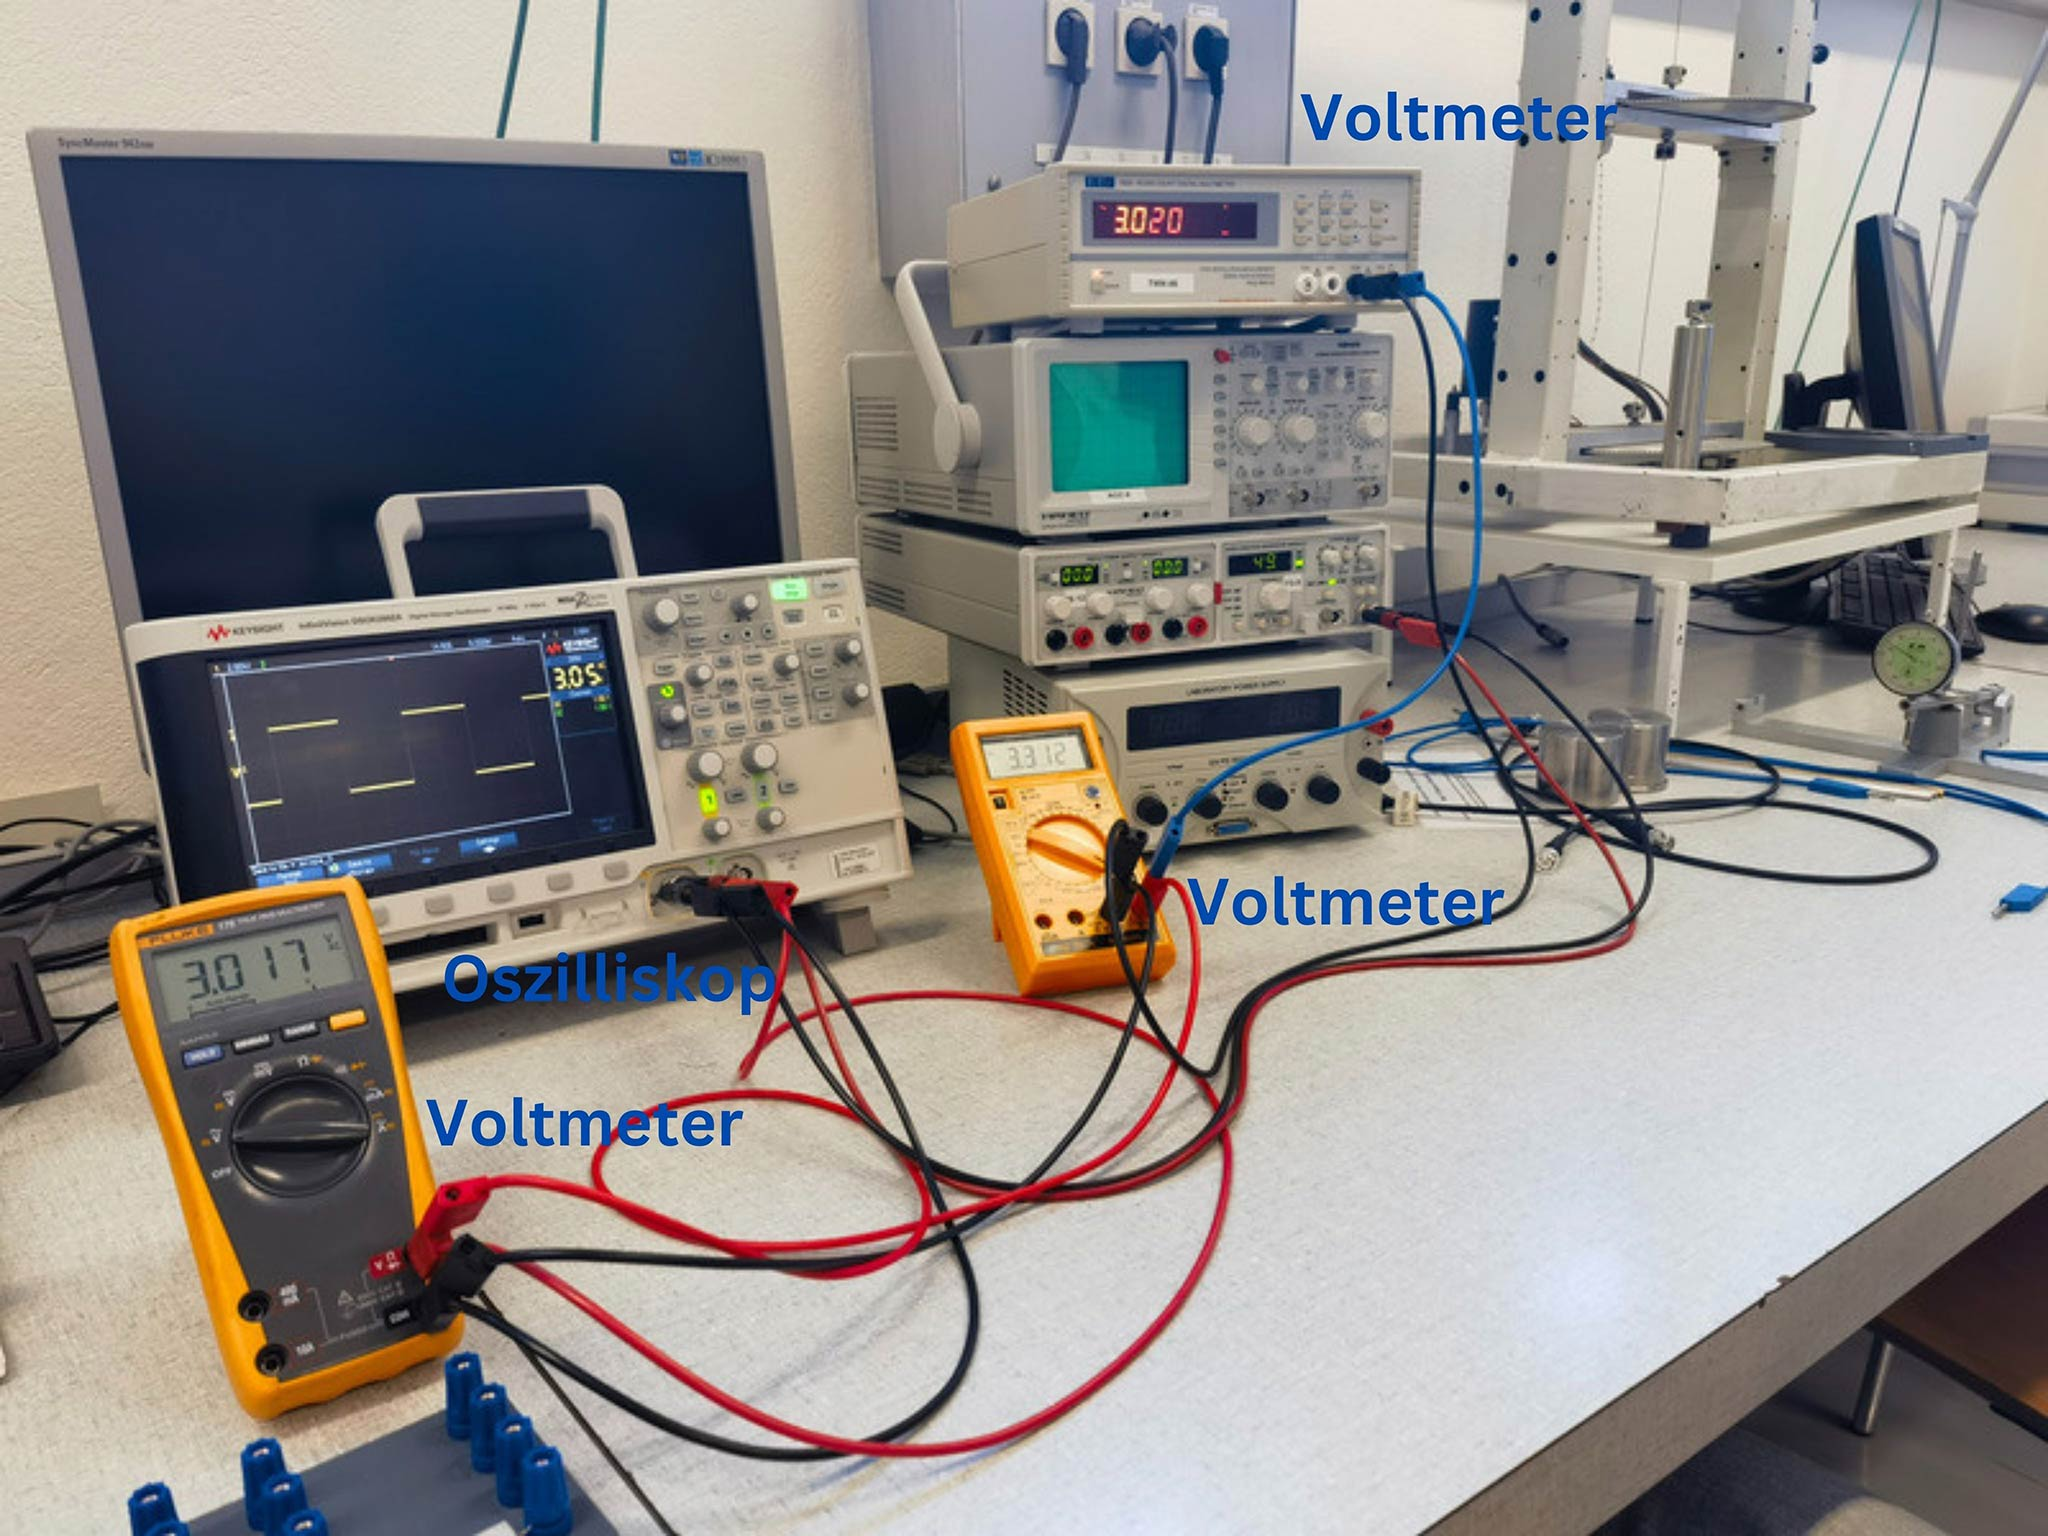
\includegraphics[width=0.4\linewidth]{nudes/PhaseLeistungBilder/Aufbau1,2.jpg}    
    \caption{Schaltplan und realer Aufbau zur Untersuchung Amplitudengänge}
    \label{fig:Aufbau2}
\end{figure}

\subsection{Phasenlage Kondensator}

Zur Bestimmung der Phasenlagen wurde zunächst für jene mit dem Kondensator folgender Aufbau vorgenommen:

\begin{figure}[H]
    \centering
    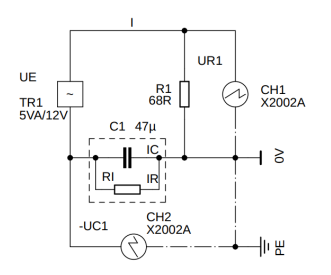
\includegraphics[width=0.4\linewidth]{nudes/Schaltplan3.PNG}
    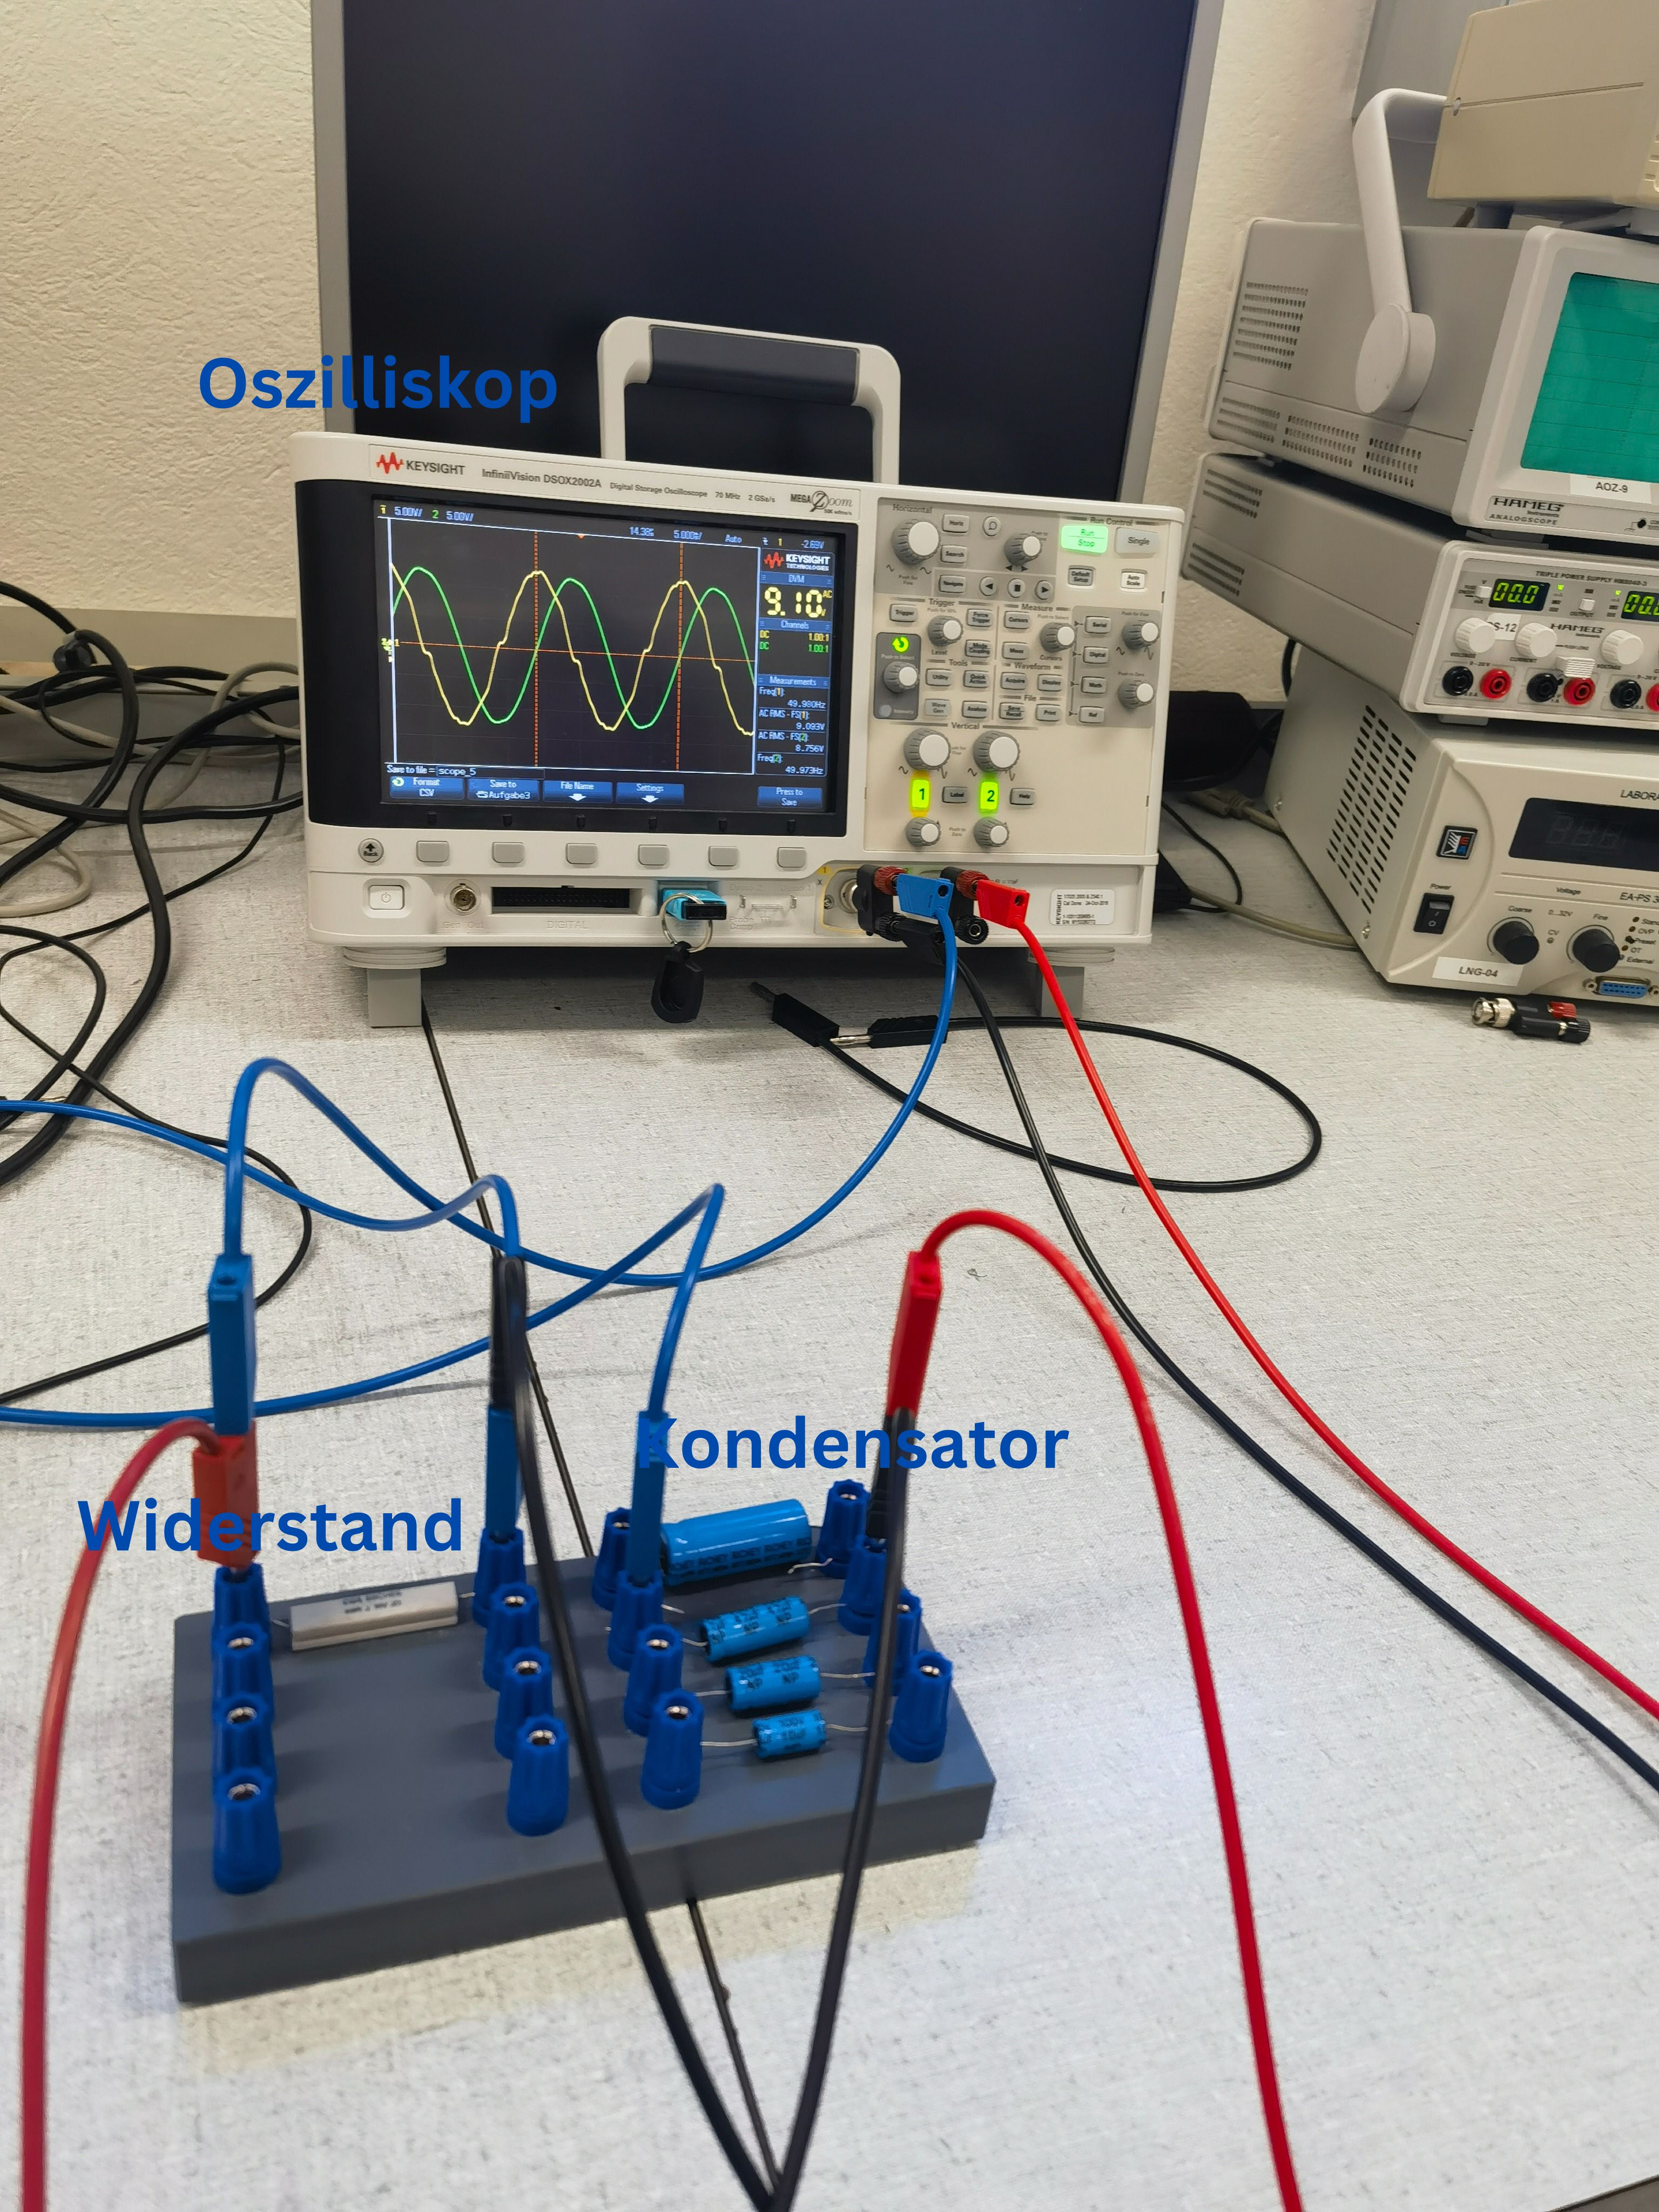
\includegraphics[width=0.4\linewidth]{nudes/PhaseLeistungBilder/Aufbau3.jpg}
    \caption{Schaltplan und realer Aufbau zur Bestimmung der Phasenlage des Kondensators}
    \label{fig:Aufbau3}
\end{figure}

\subsection{Phasenlage Spule}

Selbiger Aufbau, jedoch mit einer Spule anstelle des Kondensators wurde dann beim nächsten Versuchspunkt realisiert.

\begin{figure}[H]
    \centering
    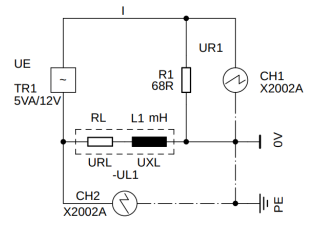
\includegraphics[width=0.4\linewidth]{nudes/Schaltplan4.PNG}
    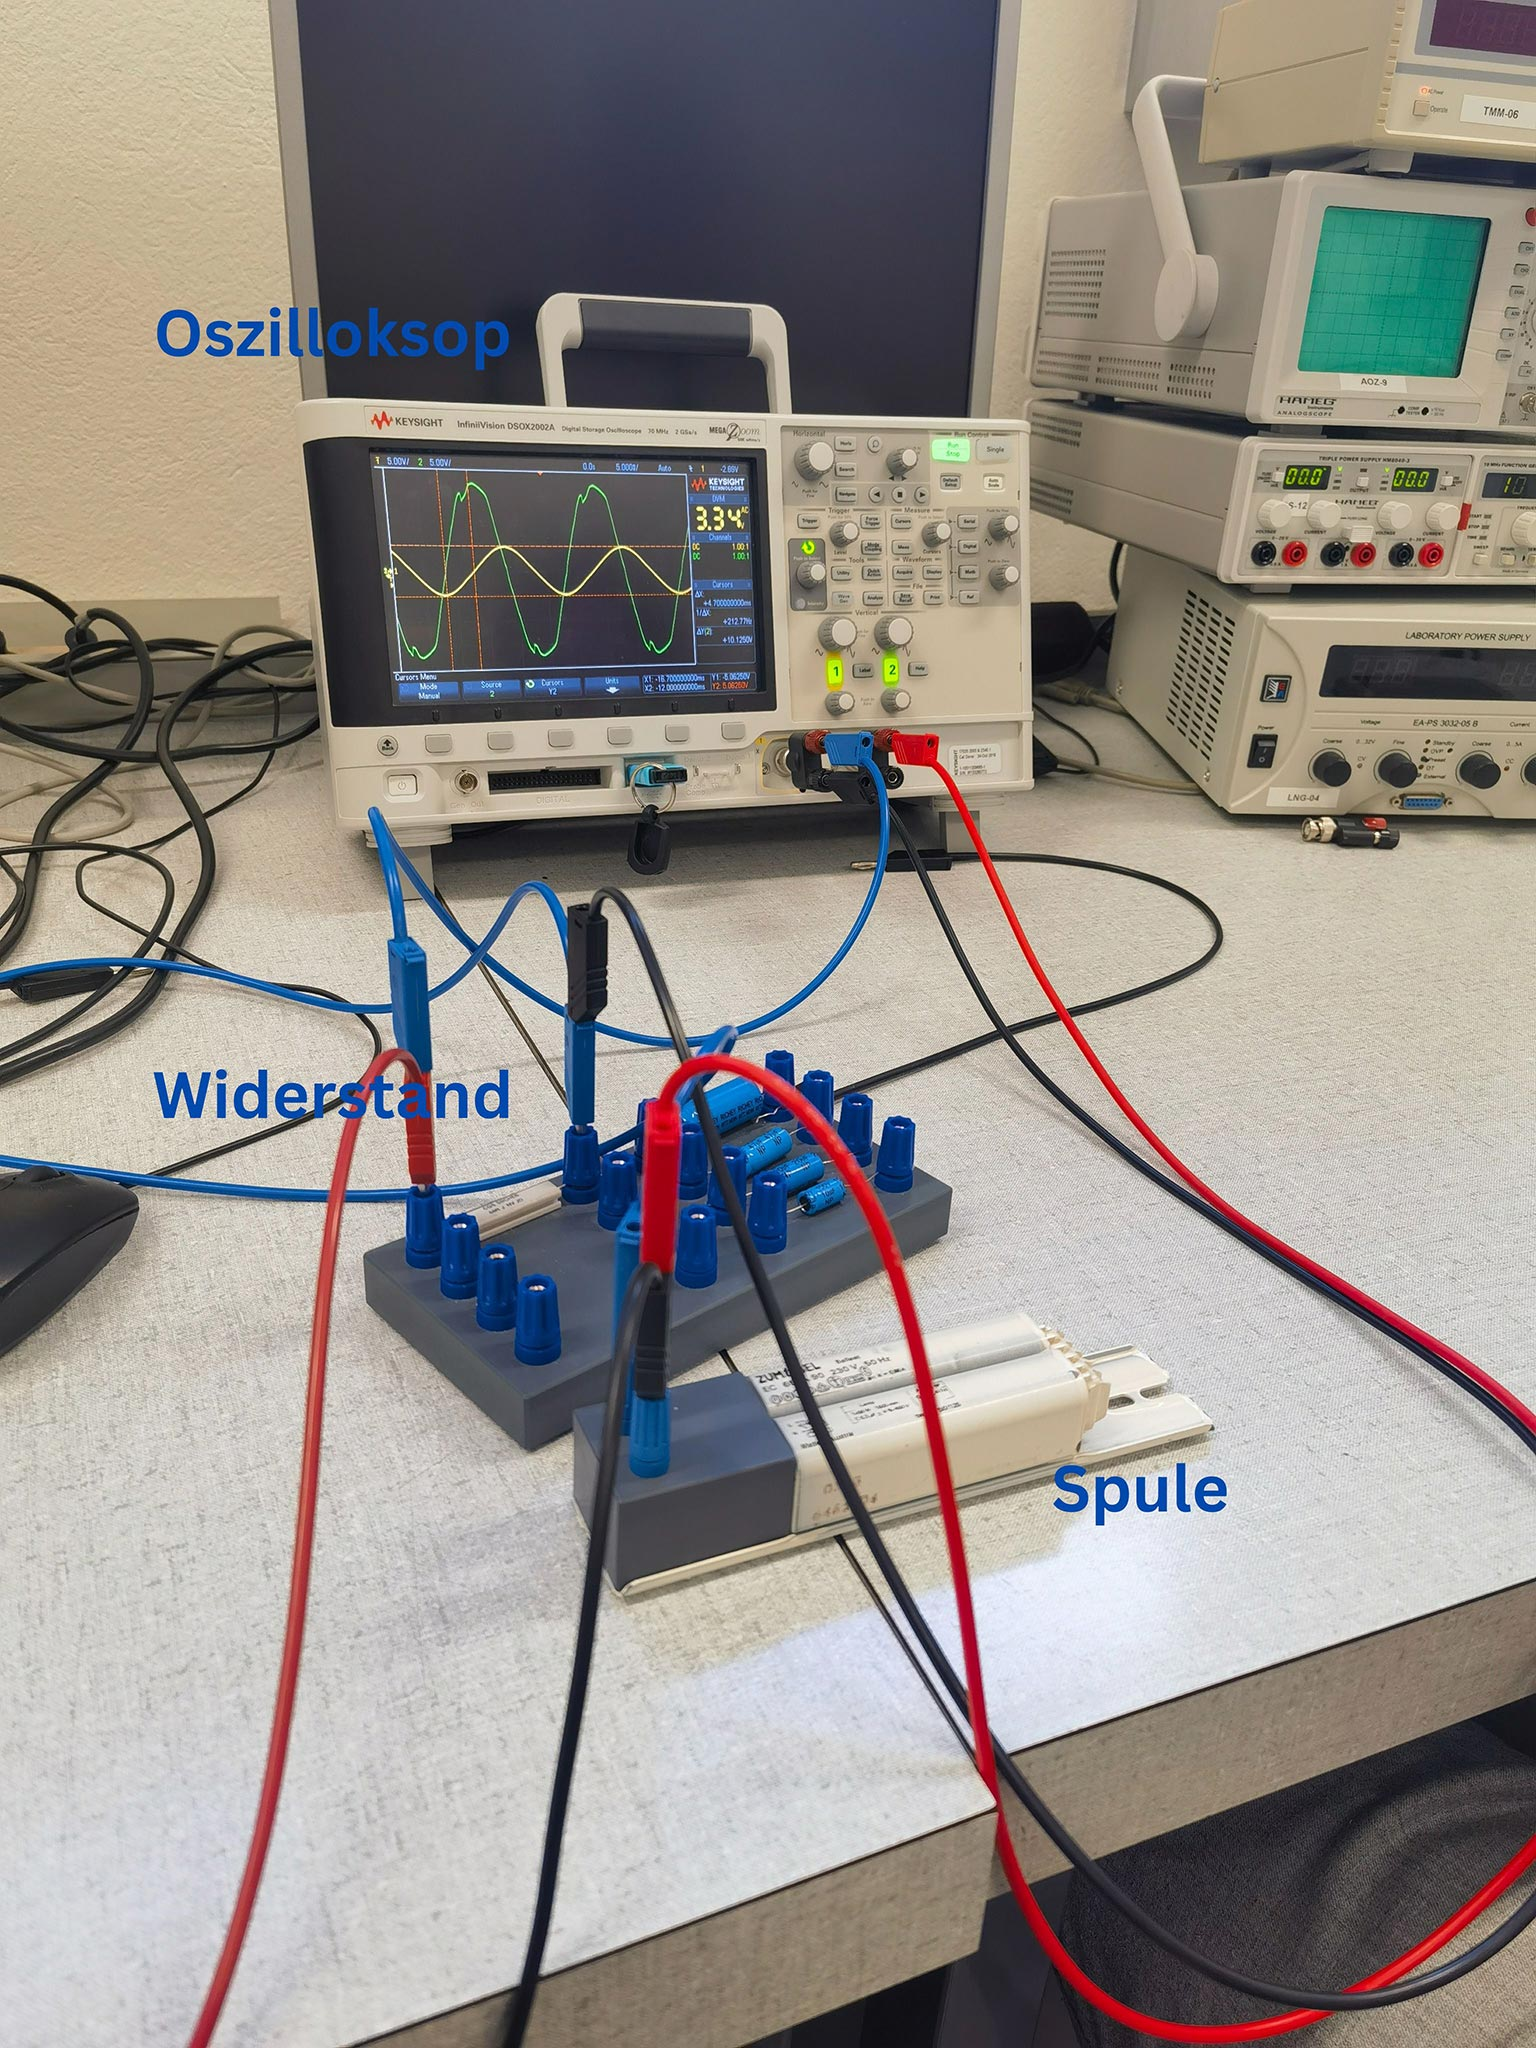
\includegraphics[width=0.4\linewidth]{nudes/PhaseLeistungBilder/Aufbau4.jpg}
    \caption{Schaltplan und realer Aufbau zur Bestimmung der Phasenlage der Spule}
    \label{fig:Aufbau4}
\end{figure}

\subsection{Elektrische Leistung RC-Schaltung}

Zur Bestimmung der Leistung in der RC-Schaltung wurde folgender Schaltplan in die Tat umgesetzt:

\begin{figure}[H]
    \centering
    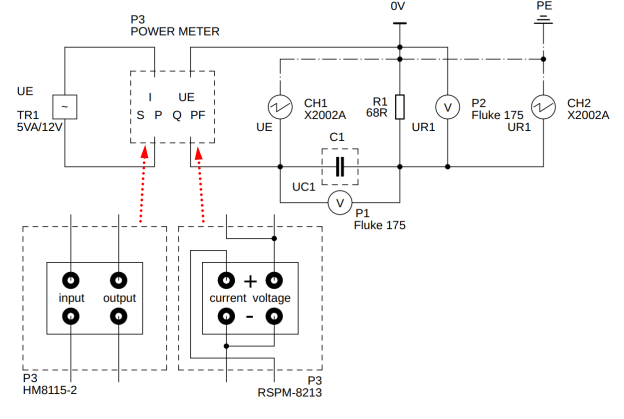
\includegraphics[width=0.4\linewidth]{nudes/Schaltplan5.PNG}
    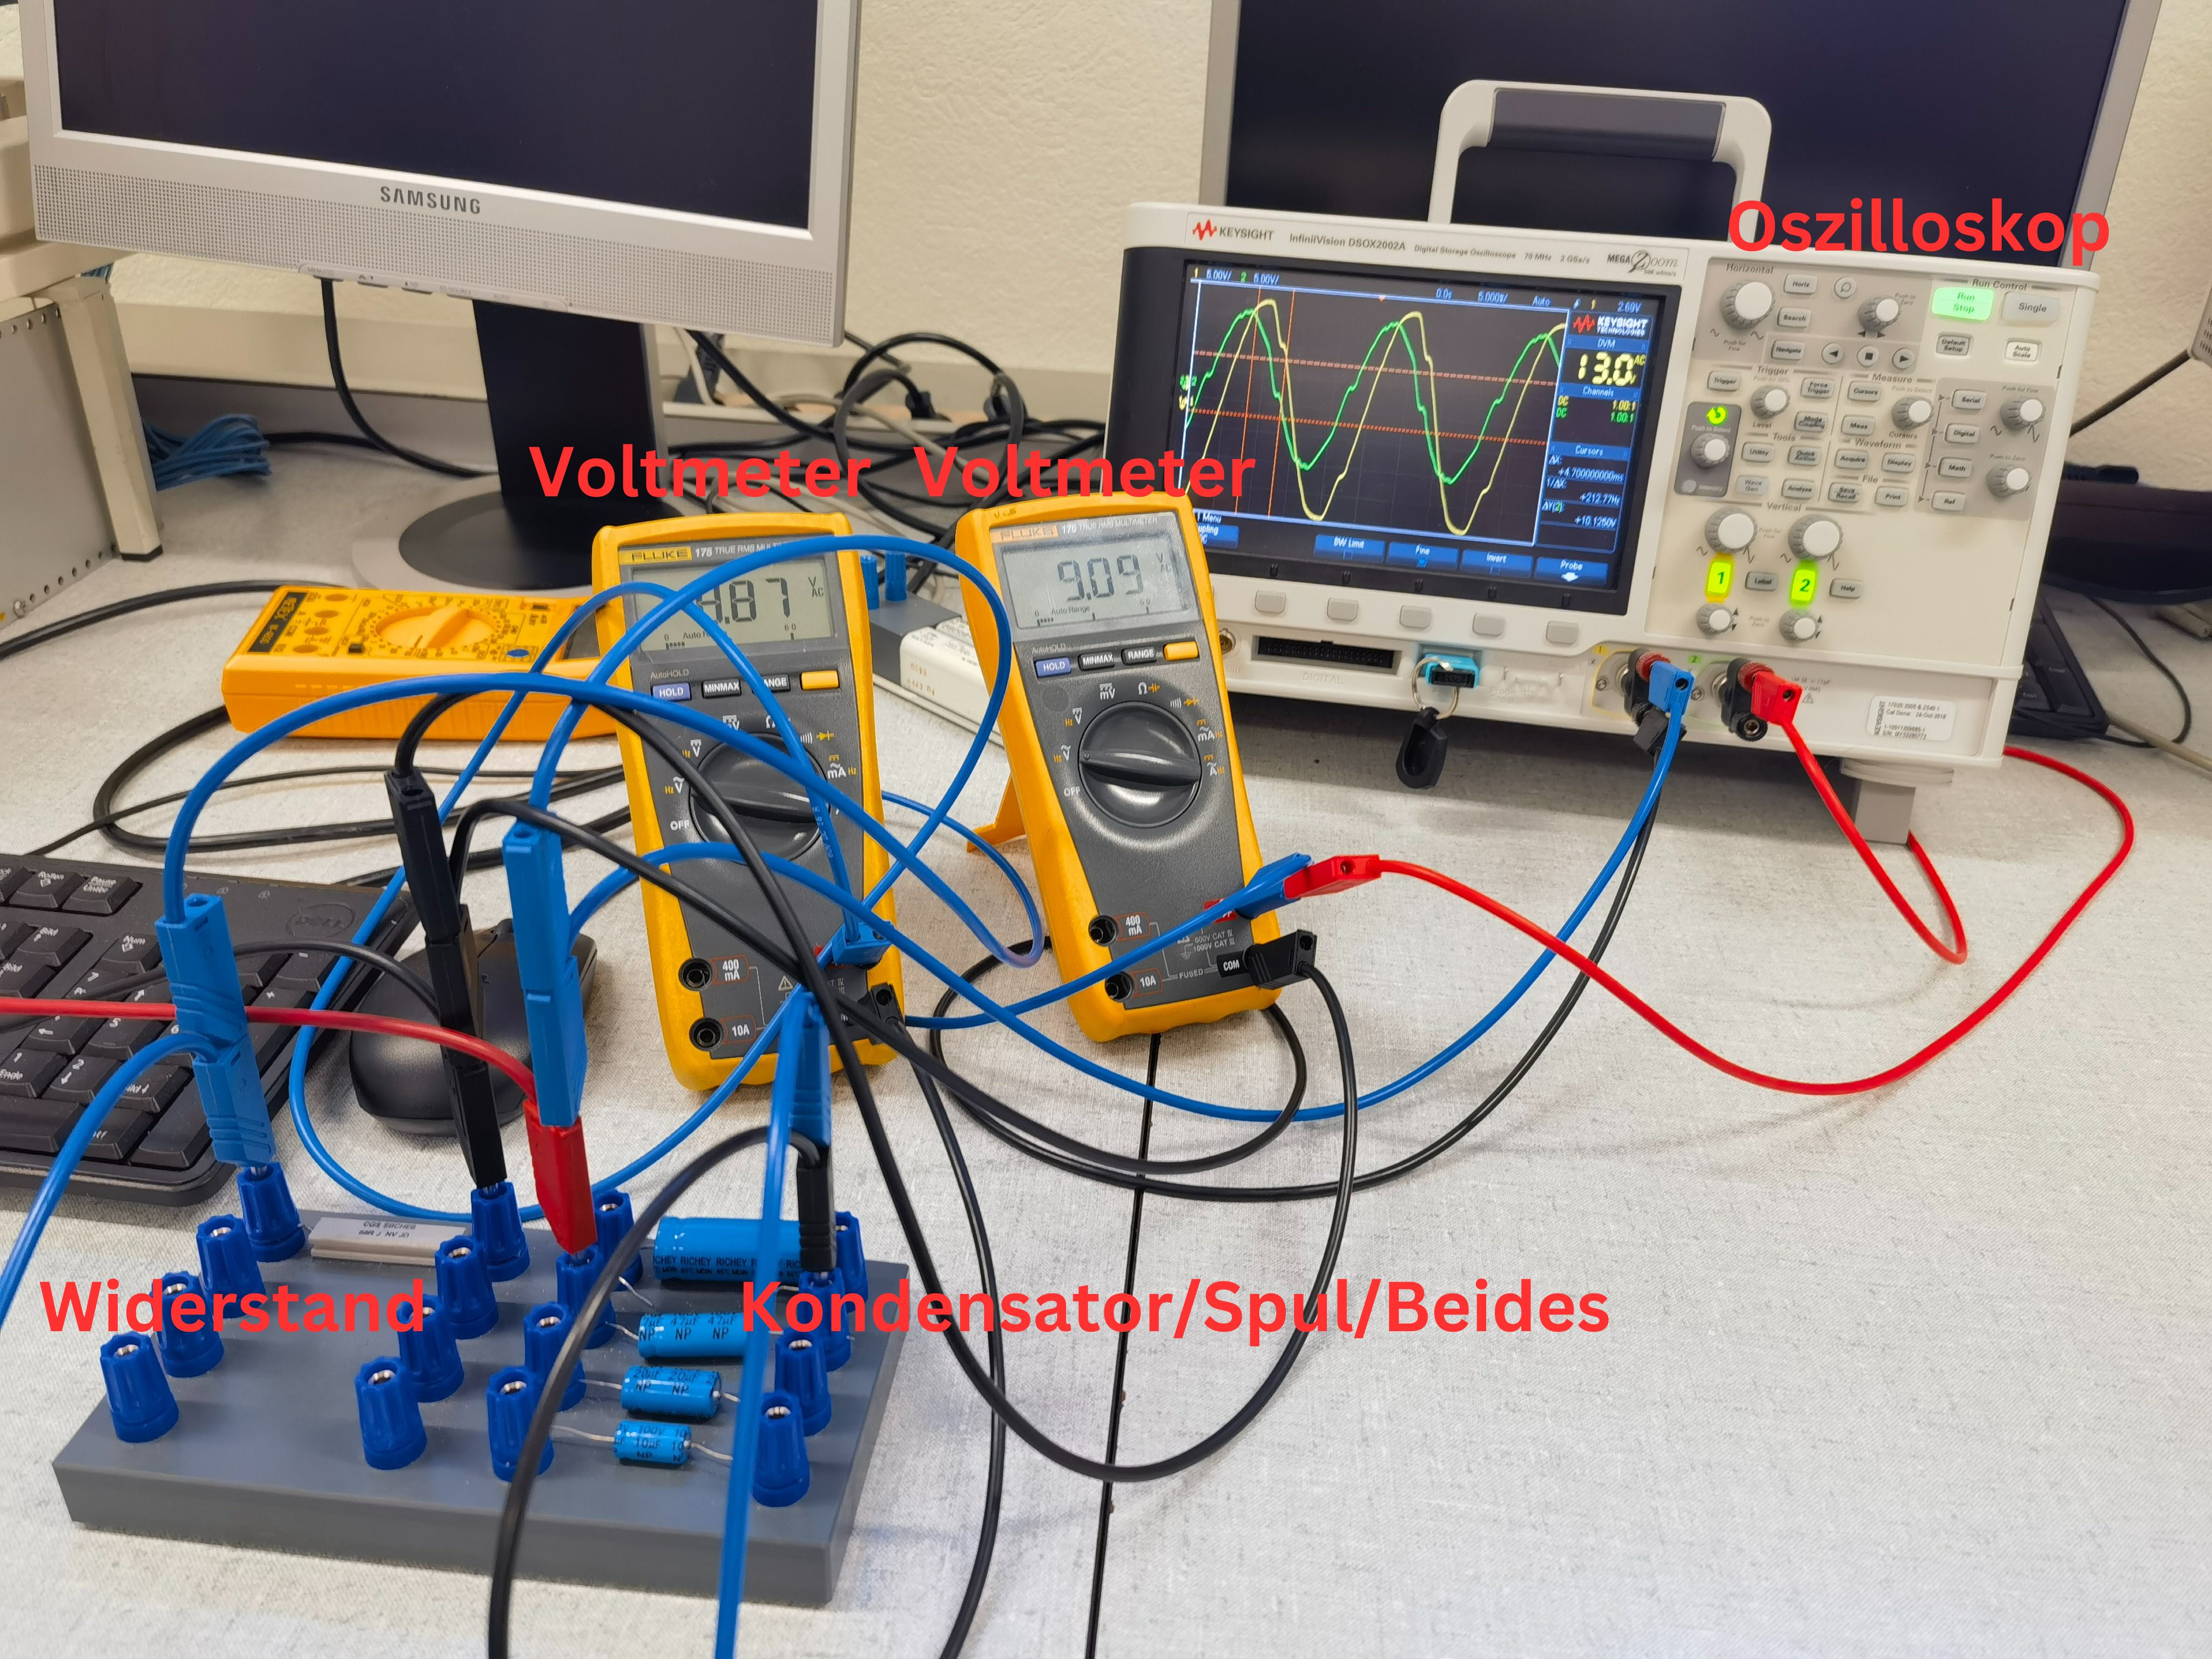
\includegraphics[width=0.4\linewidth]{nudes/PhaseLeistungBilder/Aufbau5,6,7.jpg}
    \caption{Schaltplan und realer Aufbau zur Bestimmung der elektrischen Leistung der RC-Schaltung}
    \label{fig:Aufbau5}
\end{figure}

\noindent
Für die letzten drei Aufgabenpunkte wurde außerdem ein Trafo und ein PowerMeter zur Spannungsversorgung verwendet:

\begin{figure}[H]
    \centering
    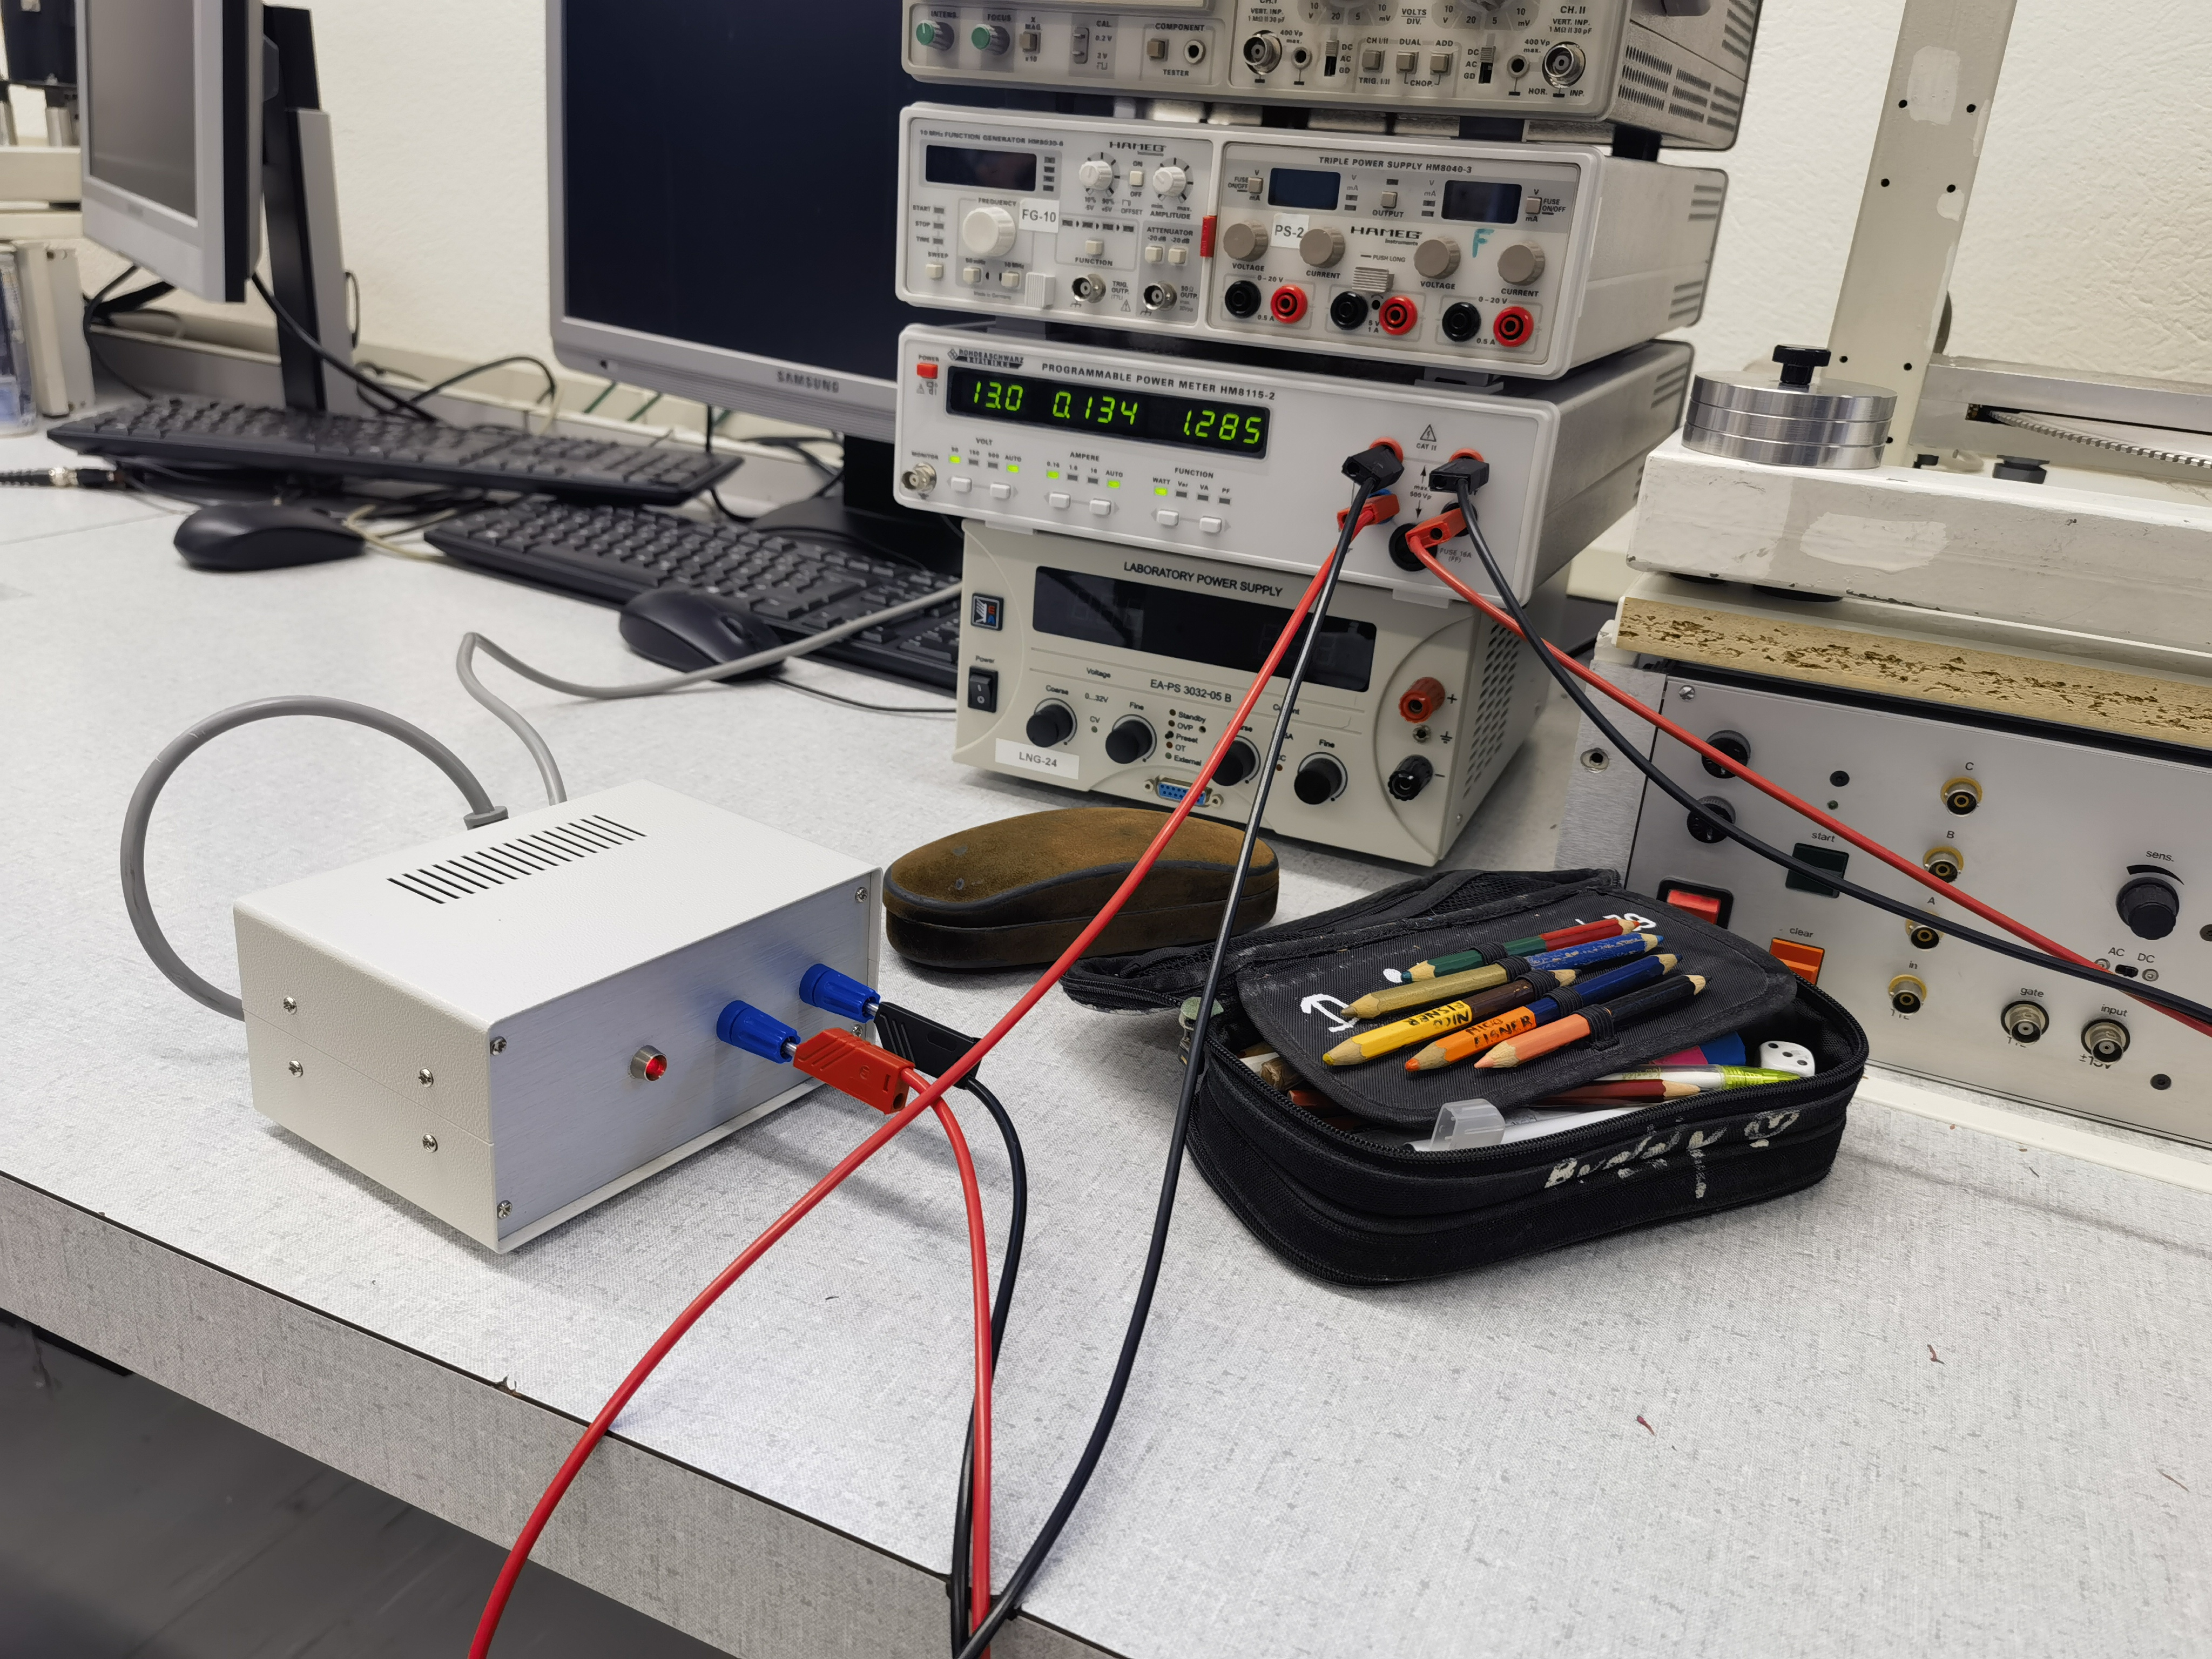
\includegraphics[width=0.4\linewidth]{nudes/PhaseLeistungBilder/Trafo,Powermeter.jpg}
    \caption{Trafo und Powermeter}
    \label{fig:TrafoPowerMeter}
\end{figure}


\subsection{Elektrische Leistung RL-Schaltung}

Mit der selben Spannungsversorgung wie in vorheriger Aufgabe wurde dann die RL-Schaltung aufgebaut:

\begin{figure}[H]
    \centering
    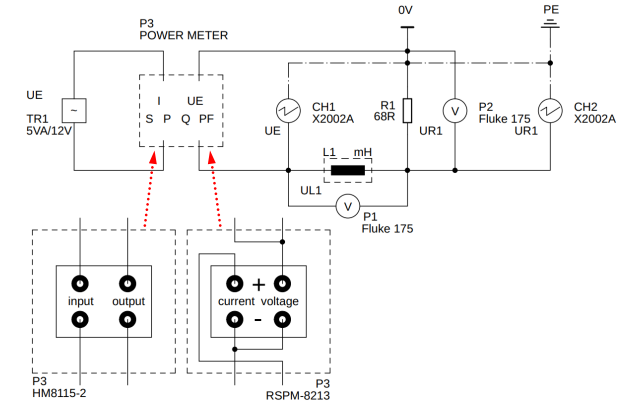
\includegraphics[width=0.4\linewidth]{nudes/Schaltplan6.PNG}
    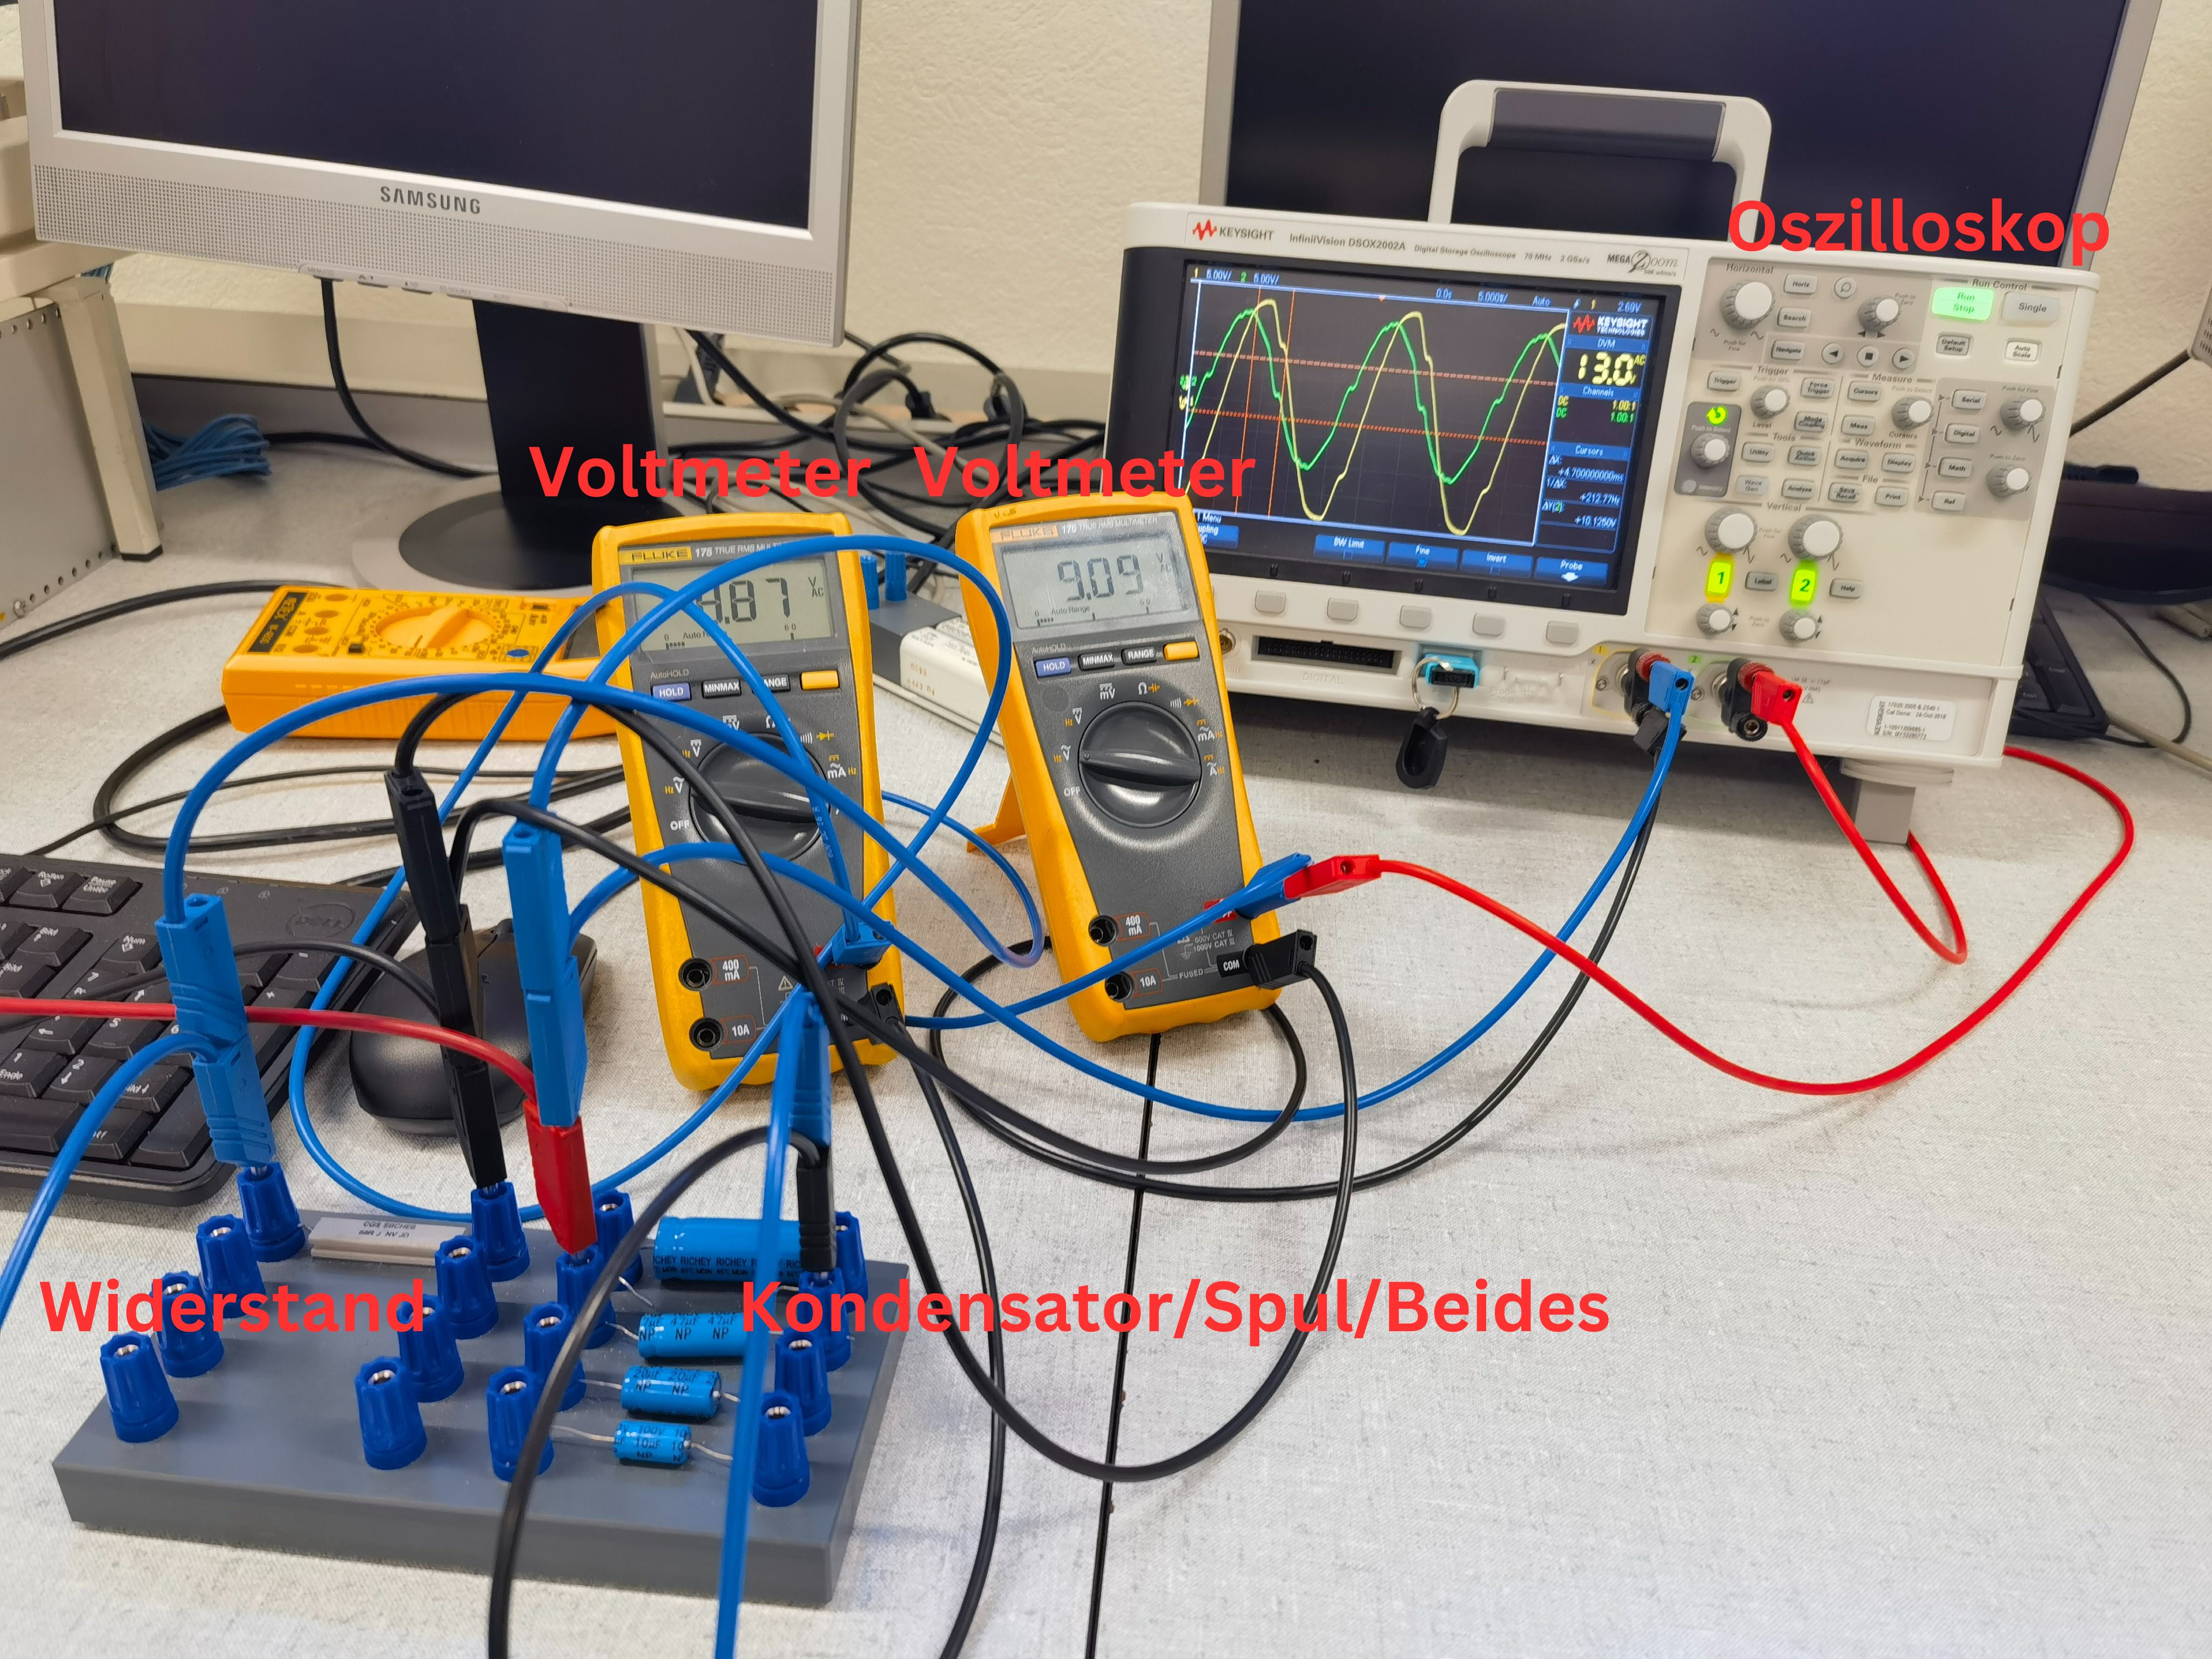
\includegraphics[width=0.4\linewidth]{nudes/PhaseLeistungBilder/Aufbau5,6,7.jpg}
    \caption{Schaltplan und realer Aufbau zur Bestimmung der elektrischen Leistung der RL-Schaltung}
    \label{fig:Aufbau6}
\end{figure}



\subsection{Blindleistungskompensation}

Beim experimentieren mit der Blindleistungskompensation wurden dann eine Kapazität und eine Spule gemeinsam in den Schaltkreis eingebunden:

\begin{figure}[H]
    \centering
    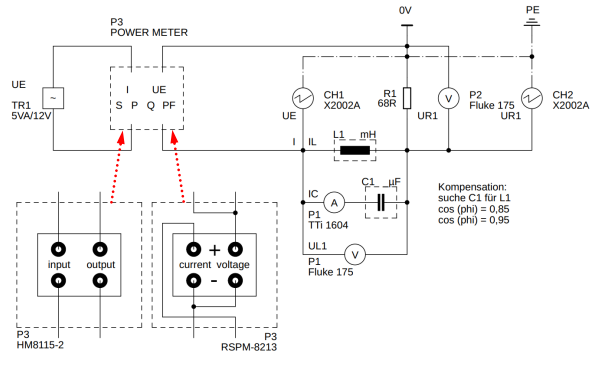
\includegraphics[width=0.4\linewidth]{nudes/Schaltplan7.PNG}
    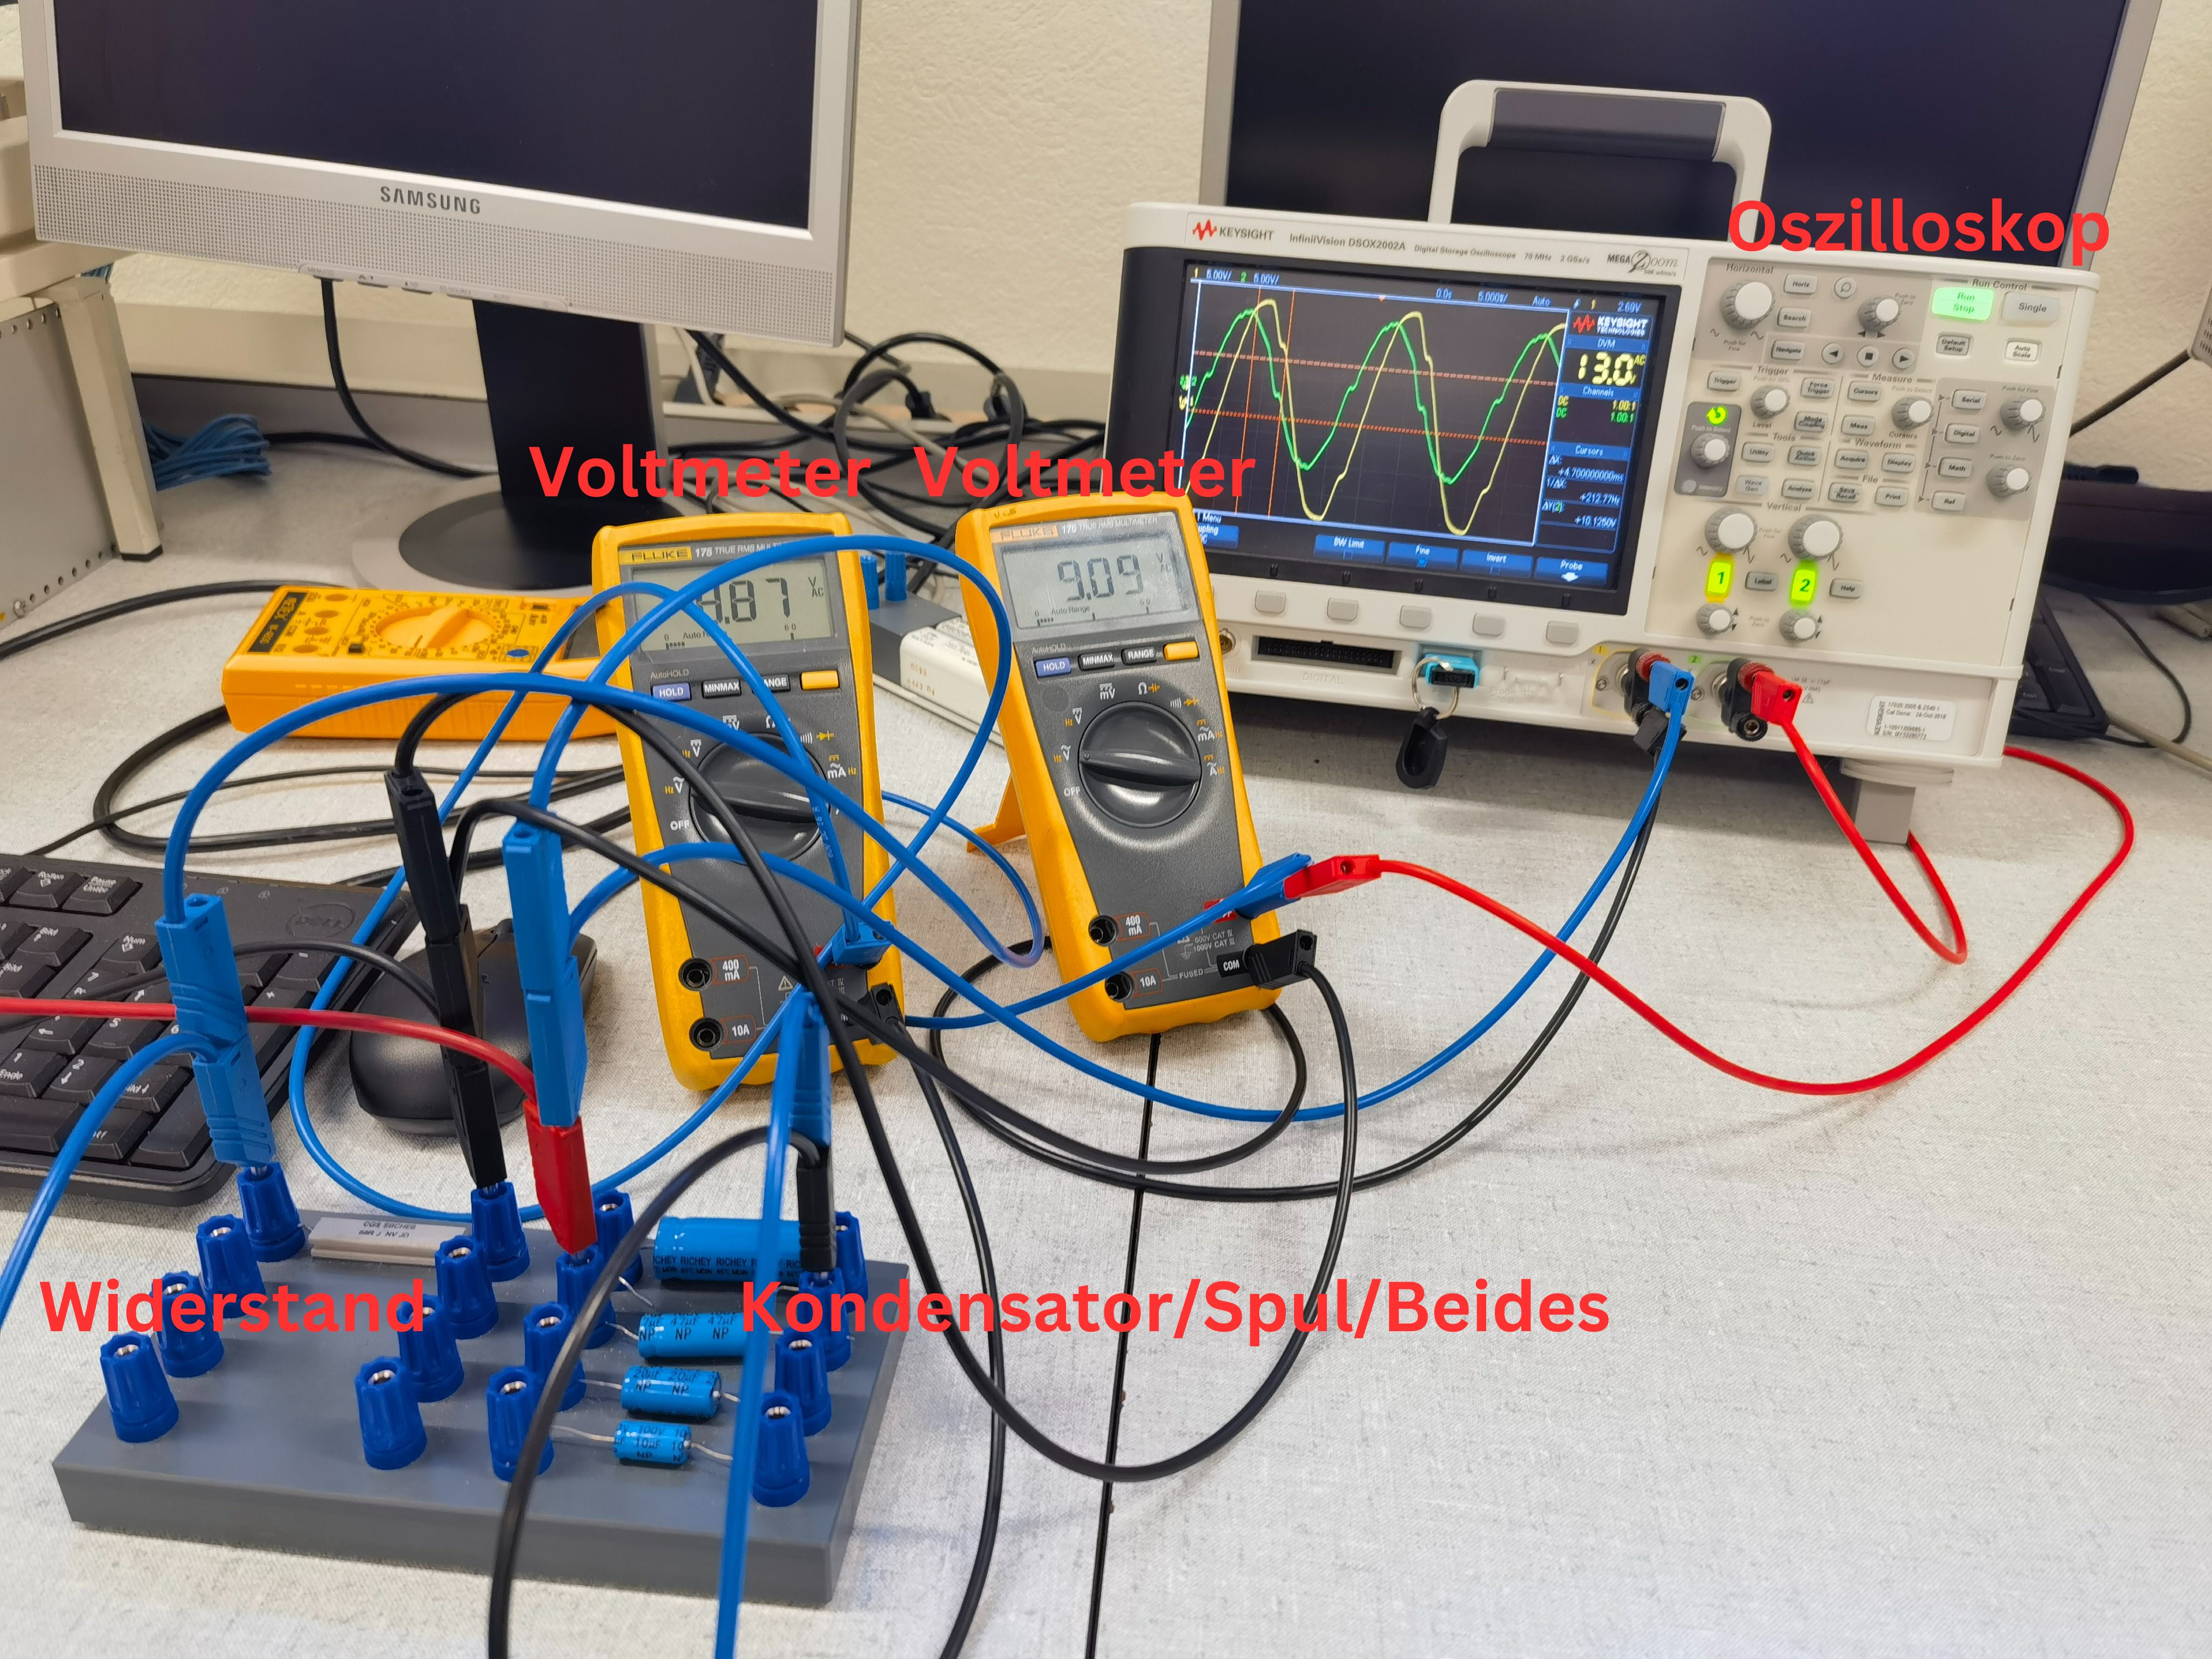
\includegraphics[width=0.4\linewidth]{nudes/PhaseLeistungBilder/Aufbau5,6,7.jpg}
    \caption{Schaltplan und realer Aufbau zur Untersuchung der Blindleistungskompensation}
    \label{fig:Aufbau7}
\end{figure}



\section{Geräteliste} %jo holt a listn ------------------------------

    \begin{table}[H]
        \centering
        \caption{Im Versuch verwendete Geräte und Utensilien.}
        \label{tab:geraete}
        \resizebox{\columnwidth}{!}{\begin{tabular}{|l|l|l|l|l|l|l|}
            \hline
            Gerät   & Gerät  & Unsicherheit \\
            \hline
            Funktionsgenerator & HM8030 & {n.a} \\
            Leistungsmessgerät & HM8030 & $\pm$ 0.8$\%$ + 10 dig P / $\pm$ 2.5$\%$ + 10 dig Q / $\pm$ 0.8$\%$ + 5 dig S / $\pm$ 2$\%$ + 3 dig PF \\
            DMM1 & TTi 1604 & $\pm$ 0.5$\%$ + 4 dig \\
            DMM2 & Matex M-4600 & $\pm$ 0.5$\%$ + 10 dig \\
            DMM1 & Fluke 175 & $\pm$ 1.5$\%$ + 3 dig \\
            Oszilloskop & Keysight DSO-X 2002A & $\pm$ 0.1 div \\
            Trafo & {n.a} & {n.a} \\
            Widerstand & 68 $\Omega$ & {n.a} \\
            Kondensatoren & 10, 20, 47, 100 $\mu F$ & {n.a} \\
            Spule & Zumtobel & {n.a} \\
            \hline    
        \end{tabular}}
    \end{table}


\section{Versuchsdurchführung \& Messergebnisse} %nachvollziehbar und klar dargestellt ------------------------------


\subsection{Untersuchung der Anzeigen}

Um die verschiedenen Messgeräte auf Anzeigefehler zu überprüfen, wird zunächst ein 50$\Omega$ Eingangssignal am Frequenzgenerator erzeugt und in die aufgebaute Schaltung laut Aufbauabbildung \ref{fig:Aufbau1} eingespeist.
Dabei wird eine symetrische Wechselspannung zwischen vier und acht Volt (pp) mit 50 Hz ohne DC-Anteil gewählt. Wichtig dabei ist noch das Abschwächungsverhältnis am Oszilloskop für beide Kanäle auf 1:1 zu stellen. Nun werden für den späteren Vergleich Messdaten verschiedener Messgeräte notiert.

\begin{table}[H]
    \centering
    \caption{Amplitudengänge Daten}
    \label{tab:Daten1}
    \begin{tabular}{| l | l | l | l |}
        \hline
        Gerät   & Sinus / V  & Dreieck / V & Rechteck / V \\
        \hline
        Oszilloskop & 2.2 $\pm$ 0.3  & 1.84 $\pm$ 0.19  & 3.1 $\pm$ 0.4 \\
        DMM 4600    & 2.22 $\pm$ 0.11 & 1.766 $\pm$ 0.018 & 3.31 $\pm$ 0.12 \\
        DMM Fluke   & 2.23 $\pm$ 0.07 & 1.84 $\pm$ 0.05 & 3.02 $\pm$ 0.08 \\
        DMMTTi      & 2.23 $\pm$ 0.06 & 1.837 $\pm$ 0.012 & 3.02 $\pm$ 0.05 \\
        \hline
    \end{tabular}
\end{table}


\subsection{Amplitudengänge}

Das Eingangssignal wie im vorherigen Teil soll nun nicht nur auf die Effektivwerte der Spannung, sondern auch mittels Oszilloskop auf Frequenz untersucht werden.
Dabei wird die Eingangsfrequenz aber nicht auf einem stabilen Wert gelassen, sondern zwischen 10 Hz - 100 kHZ variiert. 
Die daraus resultierenden Werte sind in folgender Tabelle ersichtlich:

\begin{table}[H]
    \centering
    \caption{Amplitudengänge Daten}
    \label{tab:Daten2}
    \resizebox{\columnwidth}{!}{\begin{tabular}{|l|l|l|l|l|l|l|}
        \hline
        Nr & $f_{Generator}$ / Hz & $f_{Oszi}$ / Hz & $U_{eff-Fluke}$ / V & $U_{eff-4600}$ / V & $U_{eff-TTi}$ / V & $U_{eff-Oszi}$ / V \\
        \hline
        1  & 10     & 9      & 2.2508 & 2.2140 & 2.278 & 2.219 \\
        2  & 97     & 96     & 2.2489 & 2.2400 & 2.224 & 2.239 \\
        3  & 503    & 504    & 2.2152 & 2.2340 & 2.222 & 2.238 \\
        4  & 1007   & 1008   & 2.2504 & 2.2120 & 2.228 & 2.233 \\
        5  & 2999   & 2998   & 2.2465 & 2.0450 & 2.377 & 2.231 \\
        6  & 5181   & 5183   & 2.2756 & 1.1780 & 2.698 & 2.233 \\
        7  & 10760  & 10762  & 2.2291 & 1.1760 & 2.698 & 2.233 \\
        8  & 20790  & 20792  & 2.1977 & 0.6330 & 5.734 & 2.250 \\
        9  & 25190  & 25202  & 2.2252 & 0.5526 & 6.421 & 2.262 \\
        10 & 30490  & 30466  & 2.2262 & 0.4525 & 7.101 & 2.274 \\
        11 & 35143  & 35177  & 2.2283 & 0.3873 & 7.594 & 2.284 \\
        12 & 40370  & 40391  & 2.2302 & 0.3394 & 8.045 & 2.297 \\
        13 & 45300  & 45310  & 2.2316 & 0.2890 & 8.388 & 2.309 \\
        14 & 50800  & 50779  & 2.2073 & 0.2522 & 8.686 & 2.323 \\
        15 & 55000  & 55020  & 2.2651 & 0.2287 & 8.864 & 2.335 \\
        16 & 61700  & 61742  & 2.1861 & 0.1977 & 9.112 & 2.362 \\
        17 & 66300  & 66287  & 2.2008 & 0.1806 & 9.202 & 2.378 \\
        18 & 69500  & 69512  & 2.1808 & 0.1699 & 9.244 & 2.386 \\
        19 & 75700  & 75728  & 2.1357 & 0.1520 & 9.278 & 2.406 \\
        20 & 79900  & 79921  & 2.1765 & 0.1415 & 9.274 & 2.419 \\
        21 & 84200  & 84214  & 2.1935 & 0.1311 & 9.241 & 2.435 \\
        22 & 90900  & 90901  & 2.2426 & 0.1159 & 9.149 & 2.470 \\
        23 & 93600  & 93685  & 2.2064 & 0.1103 & 9.101 & 2.489 \\
        24 & 96300  & 96377  & 2.1645 & 0.1051 & 9.046 & 2.510 \\
        25 & 100400 & 100410 & 2.1418 & 0.0979 & 8.955 & 2.547 \\
        \hline
    \end{tabular}}
\end{table}


\subsection{Phasenlage Kondensator}

Nun wird die Eingangssignalquelle gewechselt. Anstelle des Frequenzgenerators kommt ein Trafo zum Einsatz, dessen Sekundärseite nun das Signal für die neue Schaltung laut \ref{fig:Aufbau3} liefern soll.
Gemessen werden dann die Effektivwerte von $U_{R}$ und $U_{C}$, also die Spannungsabfälle am Widerstand und Kondensator, die Phasenverschiebung zwischen den beiden und eine exportierte Grafik des Messergebnisses.

\begin{table}[H]
    \centering
    \caption{Phasenlage Kondensator Daten}
    \label{tab:Daten3}
    \begin{tabular}{| l | l |}
        \hline
        Messgröße & Messergebniss \\
        \hline
        $U_{pp-gelb}$ & (26.8 $\pm$ 1.3) V \\
        $U_{pp-grün}$ & (25.1 $\pm$ 1.3) V \\
        $\Delta$t & (-4.9 $\pm$ 0.5) ms \\
        \hline
    \end{tabular}
\end{table}

\noindent
Um die Spannungen auch richtig darzustellen muss Kanal 1 außerdem invertiert werden (-$U_{Ch1}$). 

\begin{figure}[H]
    \centering
    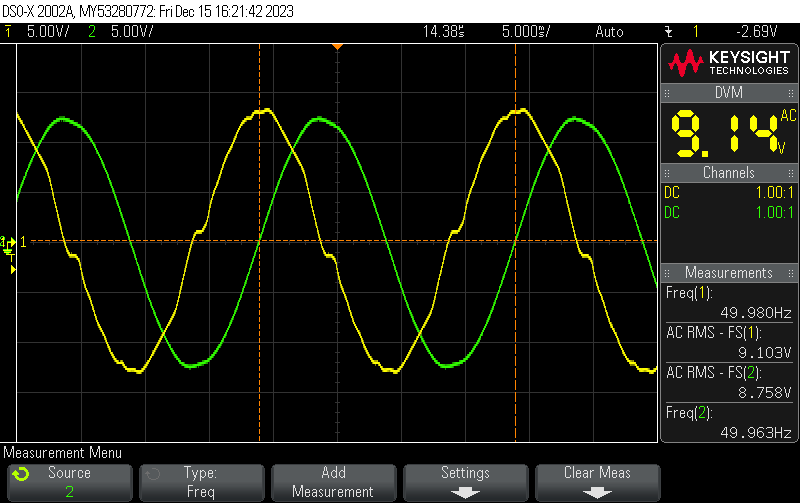
\includegraphics[width=0.6\linewidth]{nudes/PhaseLeistung/Aufgabe3/scope_3.png}
    \caption{Grafisches Messergebnis mit Kondensator}
    \label{fig:MessergebnisGrafischKondensator}
\end{figure}


\subsection{Phasenlage Spule}

Unter den selben Vorraussetzungen wie in der vorherigen Aufgabe sollen nun die gleichen Größen mit einer Spule ermittelt und festgehalten werden.
Ein weiterer Unterschied zu den vorherigen Ergebnissen ist natürlich auch, dass nun die Spannung an der Spule $U_{L}$ anstelle von $U_{C}$ resultiert.

\begin{table}[H]
    \centering
    \caption{Phasenlage Spule Daten}
    \label{tab:Daten4}
    \begin{tabular}{| l | l |}
        \hline
        Messgröße & Messergebniss \\
        \hline
        $U_{pp-gelb}$ & (10.2 $\pm$ 1.1) V \\
        $U_{pp-grün}$ & (34.9 $\pm$ 1.7) V \\
        $\Delta$t & (4.7 $\pm$ 0.5) ms  \\
        \hline
    \end{tabular}
\end{table}


\begin{figure}[H]
    \centering
    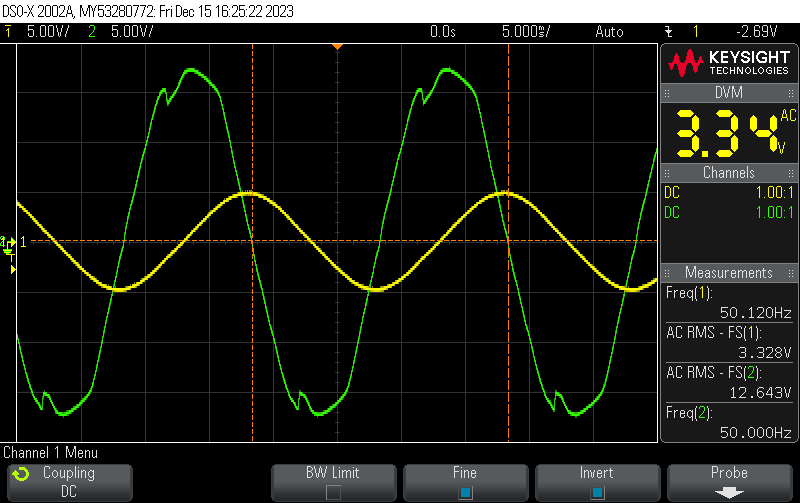
\includegraphics[width=0.6\linewidth]{nudes/PhaseLeistung/Aufgabe4/scope_6.png}
    \caption{Grafisches Messergebnis mit Spule}
    \label{fig:MessergebnisGrafischSpule}
\end{figure}


\subsection{Elektrische Leistung RC-Schaltung}

Nun wird die Schaltung zu \ref{fig:Aufbau5} umgebaut und erneut der Trafo als Spannungsquelle hinzugeschalten. Dabei sollen nun die Spannungen $U_{R1}$ an $R_{1}$ und $U_{C1}$ an $C_{1}$ gemessen werden.
Weiters soll noch der fließende Strom I und mittel PowerMeter die Wirk-, Blind- und Scheinleistung sowie der Leistungsfaktor PF notiert werden.

\begin{table}[H]
    \centering
    \caption{Elektrische Leistung RC Daten}
    \label{tab:Daten5}
    \begin{tabular}{| l | l |}
        \hline
        Messgröße & Messergebniss \\
        \hline
        U & (13.0 $\pm$ 0.2) V \\
        I & (0.134 $\pm$ 0.0015) A \\
        $U_{R}$ & (9.09 $\pm$ 0.17) V \\
        $U_{C}$ & (8.86 $\pm$ 0.09) V \\
        P & (1.286 $\pm$ 0.11) W \\
        Q & (1.18 $\pm$ 0.13) var \\
        S & (1.74 $\pm$ 0.14) VA \\
        PF & (0.740 $\pm$ 0.018) \\
        \hline
    \end{tabular}
\end{table}

\begin{figure}[H]
    \centering
    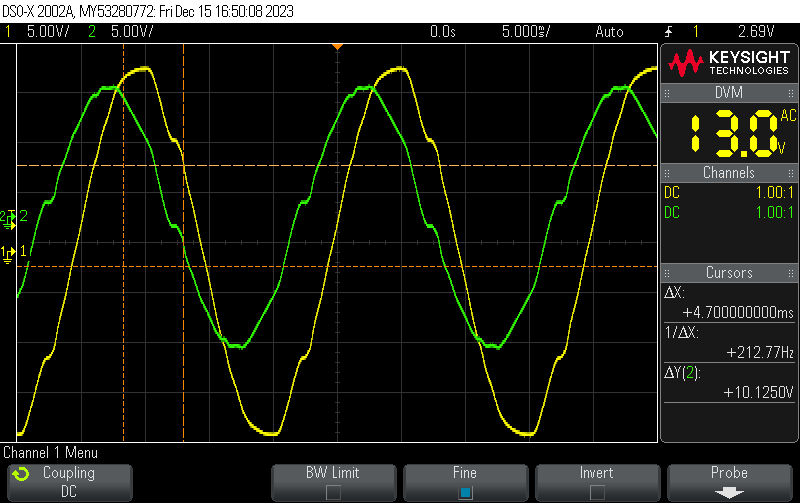
\includegraphics[width=0.6\linewidth]{nudes/PhaseLeistung/Aufgabe5/scope_7.png}
    \caption{Grafisches Messergebnis RC}
    \label{fig:MessergebnisGrafischRC}
\end{figure}


\subsection{Elektrische Leistung RL-Schaltung}

Selbiges wird nun am RL-Kreis gemessen. Hierfür wird die Schaltung wieder abgeändert und die Messung erneut gestartet.

\begin{table}[H]
    \centering
    \caption{Elektrische Leistung RL Daten}
    \label{tab:Daten6}
    \begin{tabular}{| l | l |}
        \hline
        Messgröße & Messergebniss \\
        \hline
        U & (13.6 $\pm$ 0.2) V \\
        I & (0.0500 $\pm$ 0.0007) A \\
        $U_{R}$ & (3.35 $\pm$ 0.09) V \\
        $U_{L}$ & (12.82 $\pm$ 0.11) V \\
        P & (0.245 $\pm$ 0.012) W \\
        Q & (0.630 $\pm$ 0.026) var \\
        S & (0.674 $\pm$ 0.024) VA \\
        PF & (0.360 $\pm$ 0.018) \\
        \hline
    \end{tabular}
\end{table}

\begin{figure}[H]
    \centering
    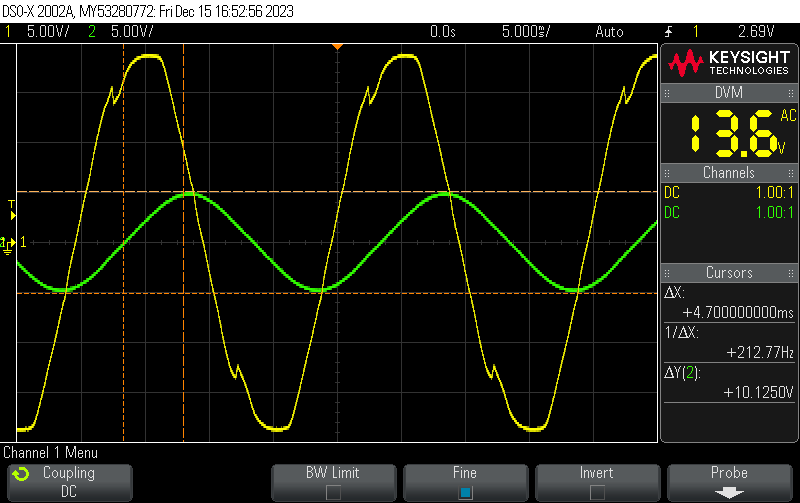
\includegraphics[width=0.6\linewidth]{nudes/PhaseLeistung/Aufgabe6/scope_11.png}
    \caption{Grafisches Messergebnis RL}
    \label{fig:MessergebnisGrafischRL}
\end{figure}



\subsection{Blindleistungskompensation}

Für die Blindleistungskompensation wird nun ein RLC-Kreis laut \ref{fig:Aufbau7} realisiert. Durch das Hinzufügen von richtig gewählten Spulen und Kondensatoren wird hier versucht, den Blindstromanteil zu verringern.
Die Schaltung wird so adjustiert, dass sich ein Powerfaktor zwischen 0.8 und 0.9 ergibt. Auch hier sollen nun die gleichen Größen wie bei den vorherhigen Kreisen plus dem Strom am Kondensator $I_{C}$ ermittelt werden.

\begin{table}[H]
    \centering
    \caption{Blindleistungskompensation Daten}
    \label{tab:Daten7}
    \begin{tabular}{| l | l |}
        \hline
        Messgröße & Messergebniss \\
        \hline
        U & (13.2 $\pm$ 0.2)V \\
        I & (0.113 $\pm$ 0.0014) A \\
        $U_{R}$ & (7.61 $\pm$ 0.08) V \\
        $U_{C}$ & (9.97 $\pm$ 0.15) V \\
        $I_{C}$ & (0.0397 $\pm 0.0009)$ A \\
        \hline
    \end{tabular}
\end{table}

\begin{figure}[H]
    \centering
    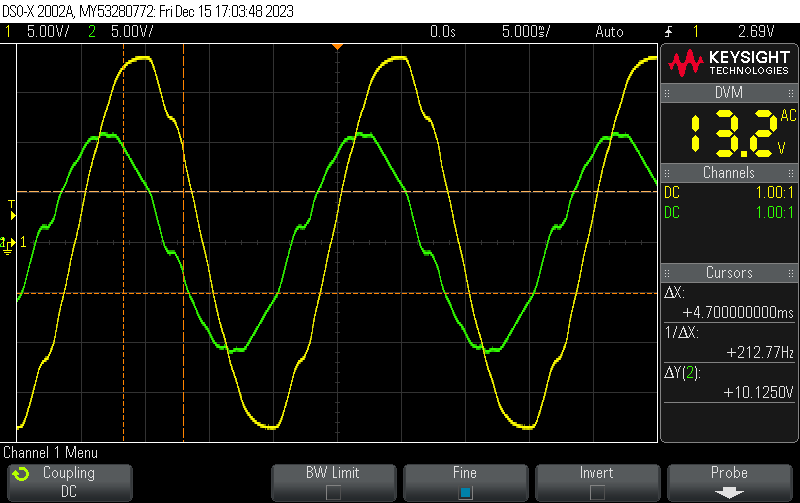
\includegraphics[width=0.6\linewidth]{nudes/PhaseLeistung/Aufgabe7/scope_14.png}
    \caption{Grafisches Messergebnis RLC}
    \label{fig:MessergebnisGrafischRLC}
\end{figure}




\section{Auswertung und Unsicherheitsanalyse} %Nicht nur zahlen angeben ------------------------------

In der Auswertung werden zur erhöhten Genauigkeit durchgehend ungerundete Werte bis zu den Endergebnissen verwendet und nur zur Darstellung gerundet. \\
Zur Berechnung der Unsicherheiten wird, wenn nicht anders angegeben, die Größtunsicherheitsmethode verwendet.

\subsection{Untersuchung der Anzeigen}

 Bei genauerer Analyse der resultierenden Daten aus Tabelle \ref{tab:Daten1} lassen sich einige Auffälligkeiten der verschiedenen Anzeigen der Spannungsmessinstrumente erkennen. \newline

\noindent
Bei den sinusförmigen Messungen lässt sich erkennen, dass alle Messgeräten unter Einbezug der Unsicherheiten auf ein gleiches Ergebnis kommen.
Bei den Dreieckssignalen sind das Oszilloskop und das Fluke in einem gemeinsamen Bereich. Das M4600 und das TTi Messgerät schwanken leicht von den anderen beiden ab.
Die Rechteckssignale wiederum werden von vom Fluke und TTi sehr ähnlich aufgenommen. Hier bilden das Oszilloskop und das M4600 die Außenseiter, wobei vor allem das M4600 etwas stärker von den anderen Werten abweicht. \newline

\noindent
Das M4600 weißt von allen die häufigsten Abweichungen auf. Dies könnte damit zusammnenhängen, dass dieses Messgerät mittels einer Analogschaltung den Gleichrichtwert bestimmt und diesen dann lediglich zum Effektivwert umrechnet. 
Für die Sinuswerte stimmt dieser Umrechnungsfaktor, bei anderen Signalformen jedoch kommt es so zu Messfehlern. 


\subsection{Amplitudengänge}

Die Amplitudengänge sind, resultierend aus den gewonnenen Daten aus Tabelle \ref{tab:Daten2}, in nachfoldender Abbildung zu erkennen.
Wichtig hierbei ist, dass sich die Amplitude aus dem Verhältnis des Ausgangs- zum Eingangssignal ergibt.
Eingangssignal ist dabei das Oszilloskopsignal, Ausgangssignale kommen von den jeweiligen Messgeräten.

\begin{figure}[H]
    \centering
    \includegraphics[width=0.6\linewidth]{nudes/AmplitudengängeGraphRichtig.jpg}
    \caption{Diagramm der Amplitudengänge in Abhängigkeit der Frequenz der verschiedenen Messinstrumente}
    \label{fig:Amplitudengänge}
\end{figure}

\noindent
Es lässt sich erkennen, dass die Amplitudengänge des Fluke stabil im Bereich des Wertes 1 Verlaufen. 
Die Verläufe des TTi und des M4600 Messgerätes verlaufen hingegen etwas anders. In den höheren Frequenzbereichen steigen sie stark an bzw. sinken stark ab.
Dies lässt darauf schließen, dass die beiden Messgeräte ab einem gewissen Frequenzbereiches nicht mehr optimale Ergebnisse liefern. 
In der Grafik lässt sich außerdem erkennen, dass dies für Frequenzen ab ungefähr 1000 Hz gilt.



\subsection{Phasenlage Kondensator}

Mit den Daten aus Tabelle \ref{tab:Daten3} lassen sich zunächst die Werte für $U_R$ und $U_C$ festlegen. \newline

\noindent
\begin{itemize}
    \item $U_R$ = (26.8 $\pm$ 1.3) V
    \item $U_C$ = (25.1 $\pm$ 1.3) V
\end{itemize}

\noindent
Mittels Gleichung \ref{eq:Phasenversatz} und dem Zeitunterschied aus Tabelle \ref{tab:Daten3} lässt sich die Phasenverschiebung ermitteln. \newline

\noindent
$\phi_C$ = (-88.2 $\pm$ 0.3) ° \newline

\noindent
Damit lässt sich nun das Zeigerdiagramm erstellen:

\begin{figure}[H]
    \centering
    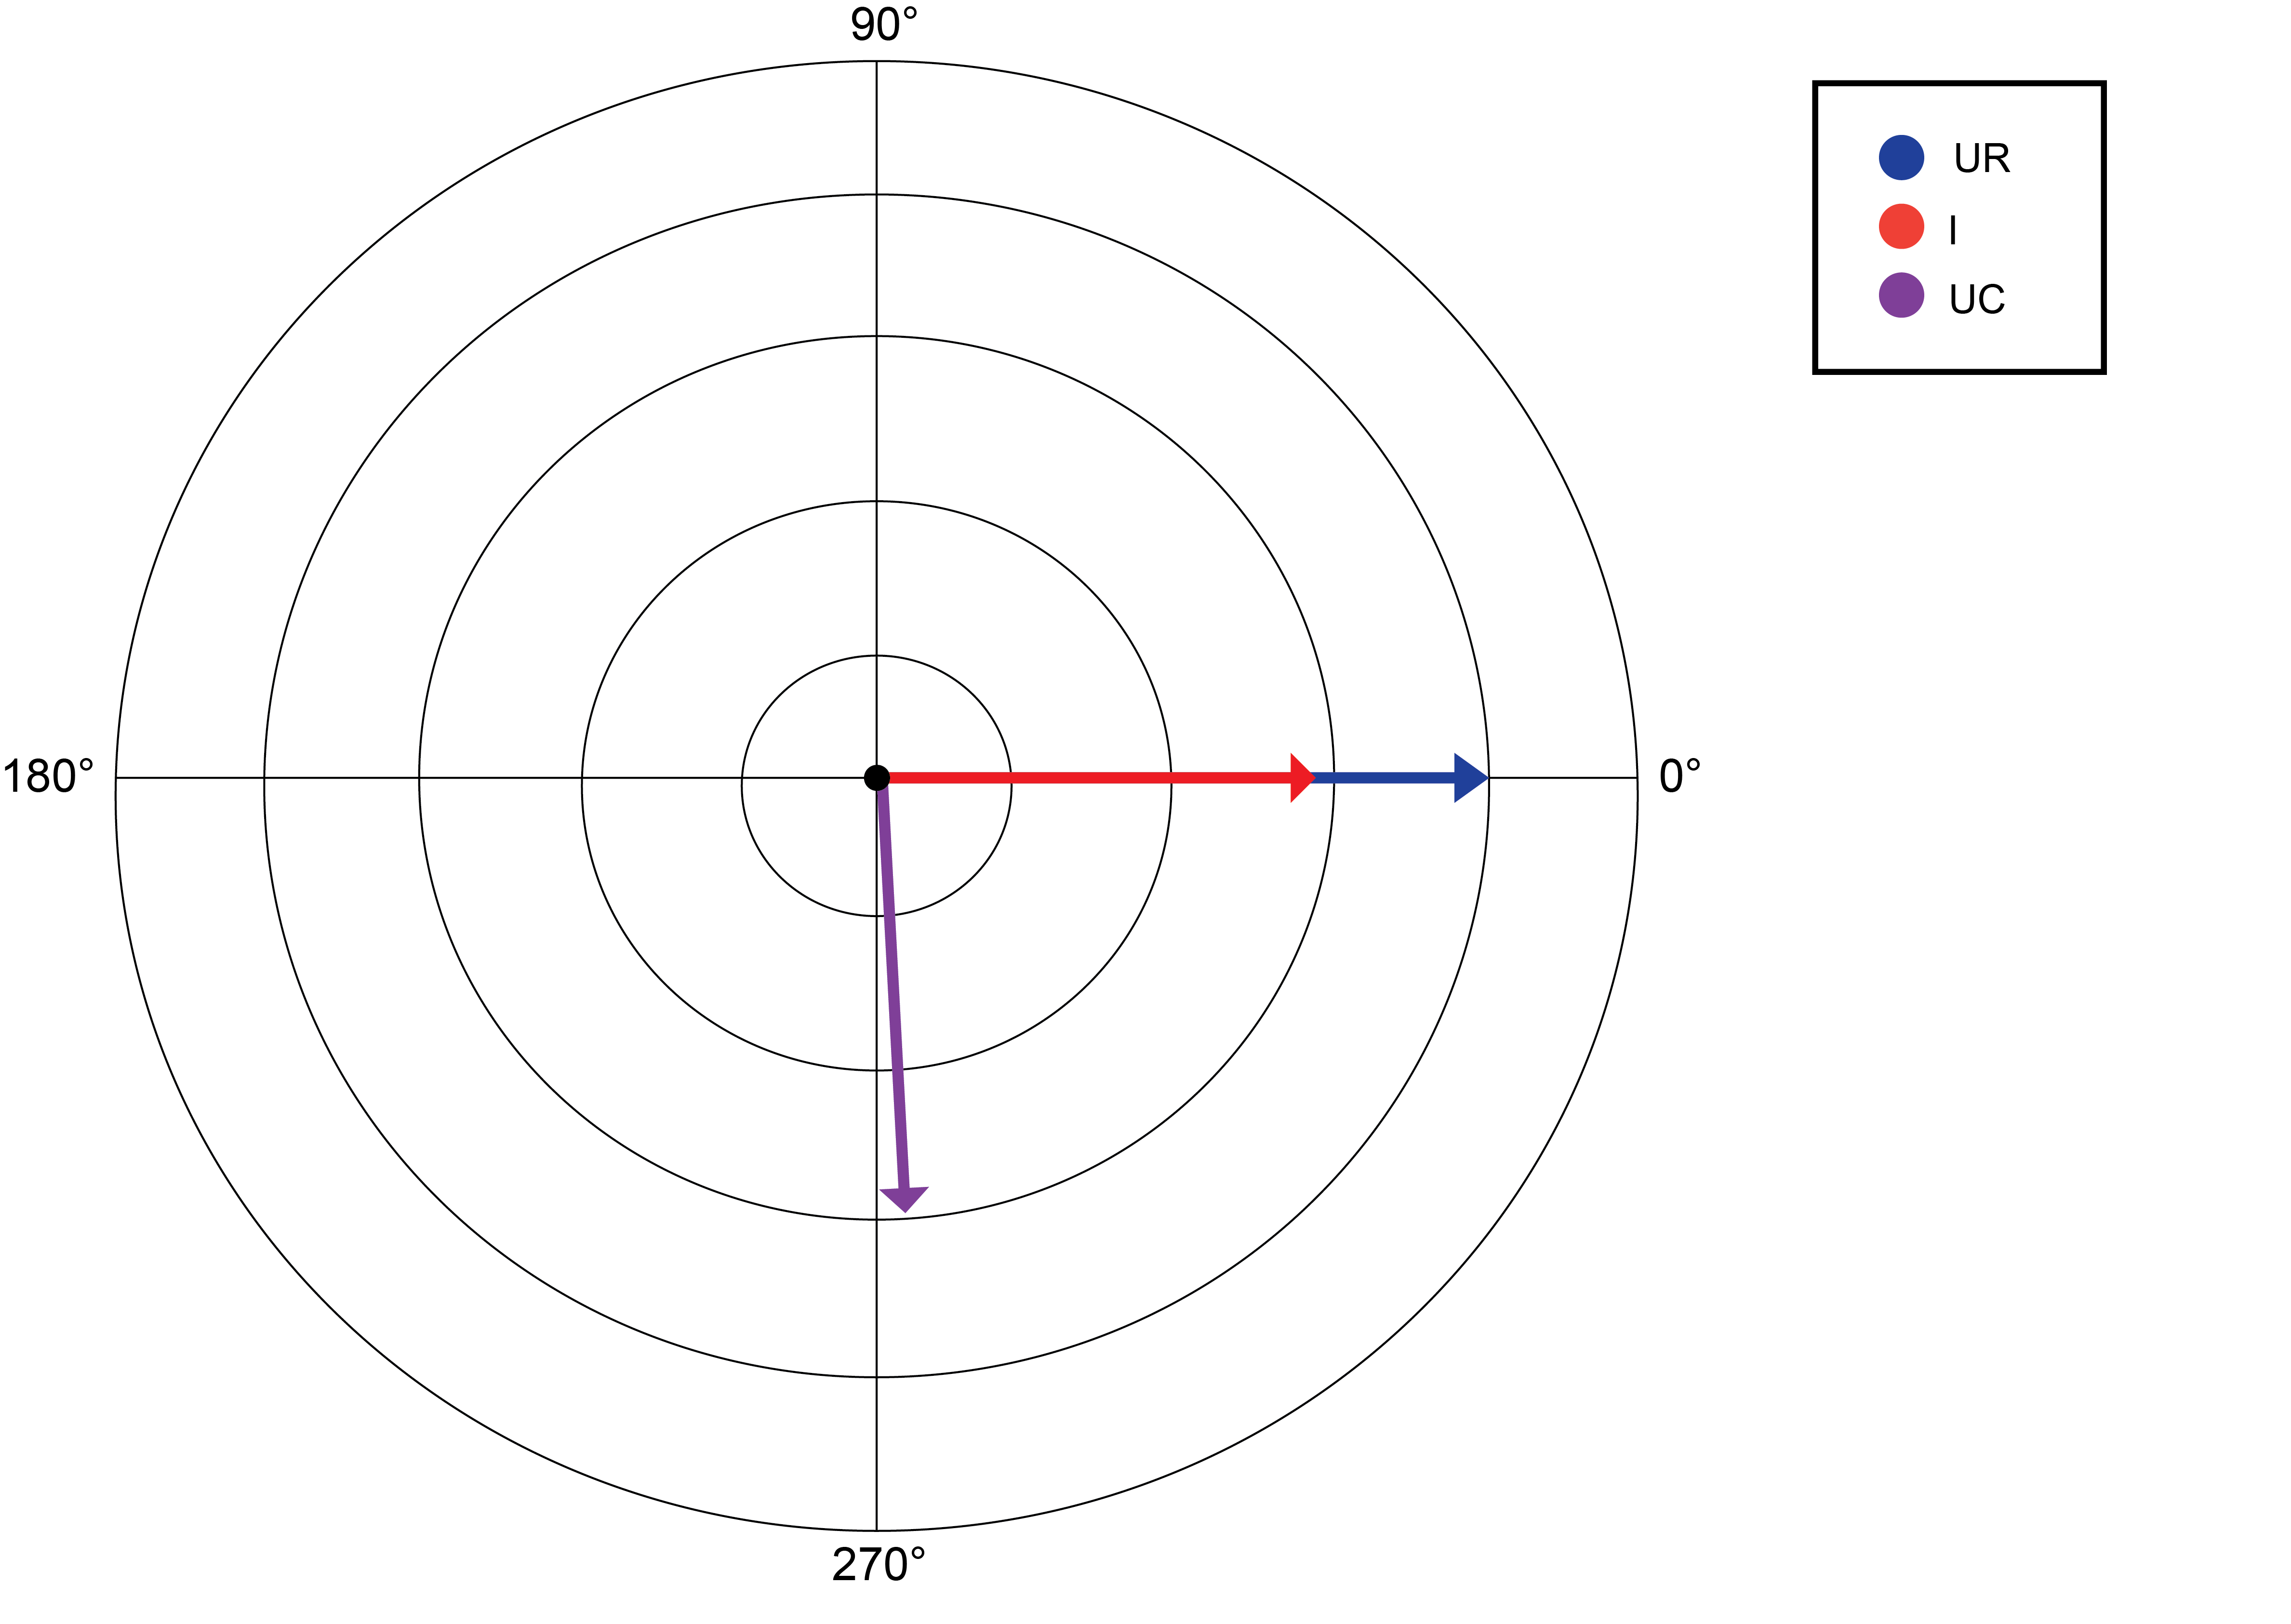
\includegraphics[width=0.6\linewidth]{nudes/Phasendiagramm3.png}
    \caption{Zeigerdiagramm der Phasenverschiebung des Kondensators}
    \label{fig:ZeigerdiagrammPhiC}
\end{figure}



\subsection{Phasenlage Spule}

Nach gleichem Prinzip nur mit den Daten aus Tabelle \ref{tab:Daten4} lassen sich nun auch die Spannung und in weiterer Folge deren Phasenlage bestimmen. \newline

\noindent
\begin{itemize}
    \item $U_R$ = (10.2 $\pm$ 1.1) V
    \item $U_L$ = (34.9 $\pm$ 1.7) V
\end{itemize}

\noindent
$\phi_L$ = (84.6 $\pm$ 0.7) ° \newline

\noindent
Daraus folgt ebenfalls ein Zeigerdiagramm mit den berechneten Größen.

\begin{figure}[H]
    \centering
    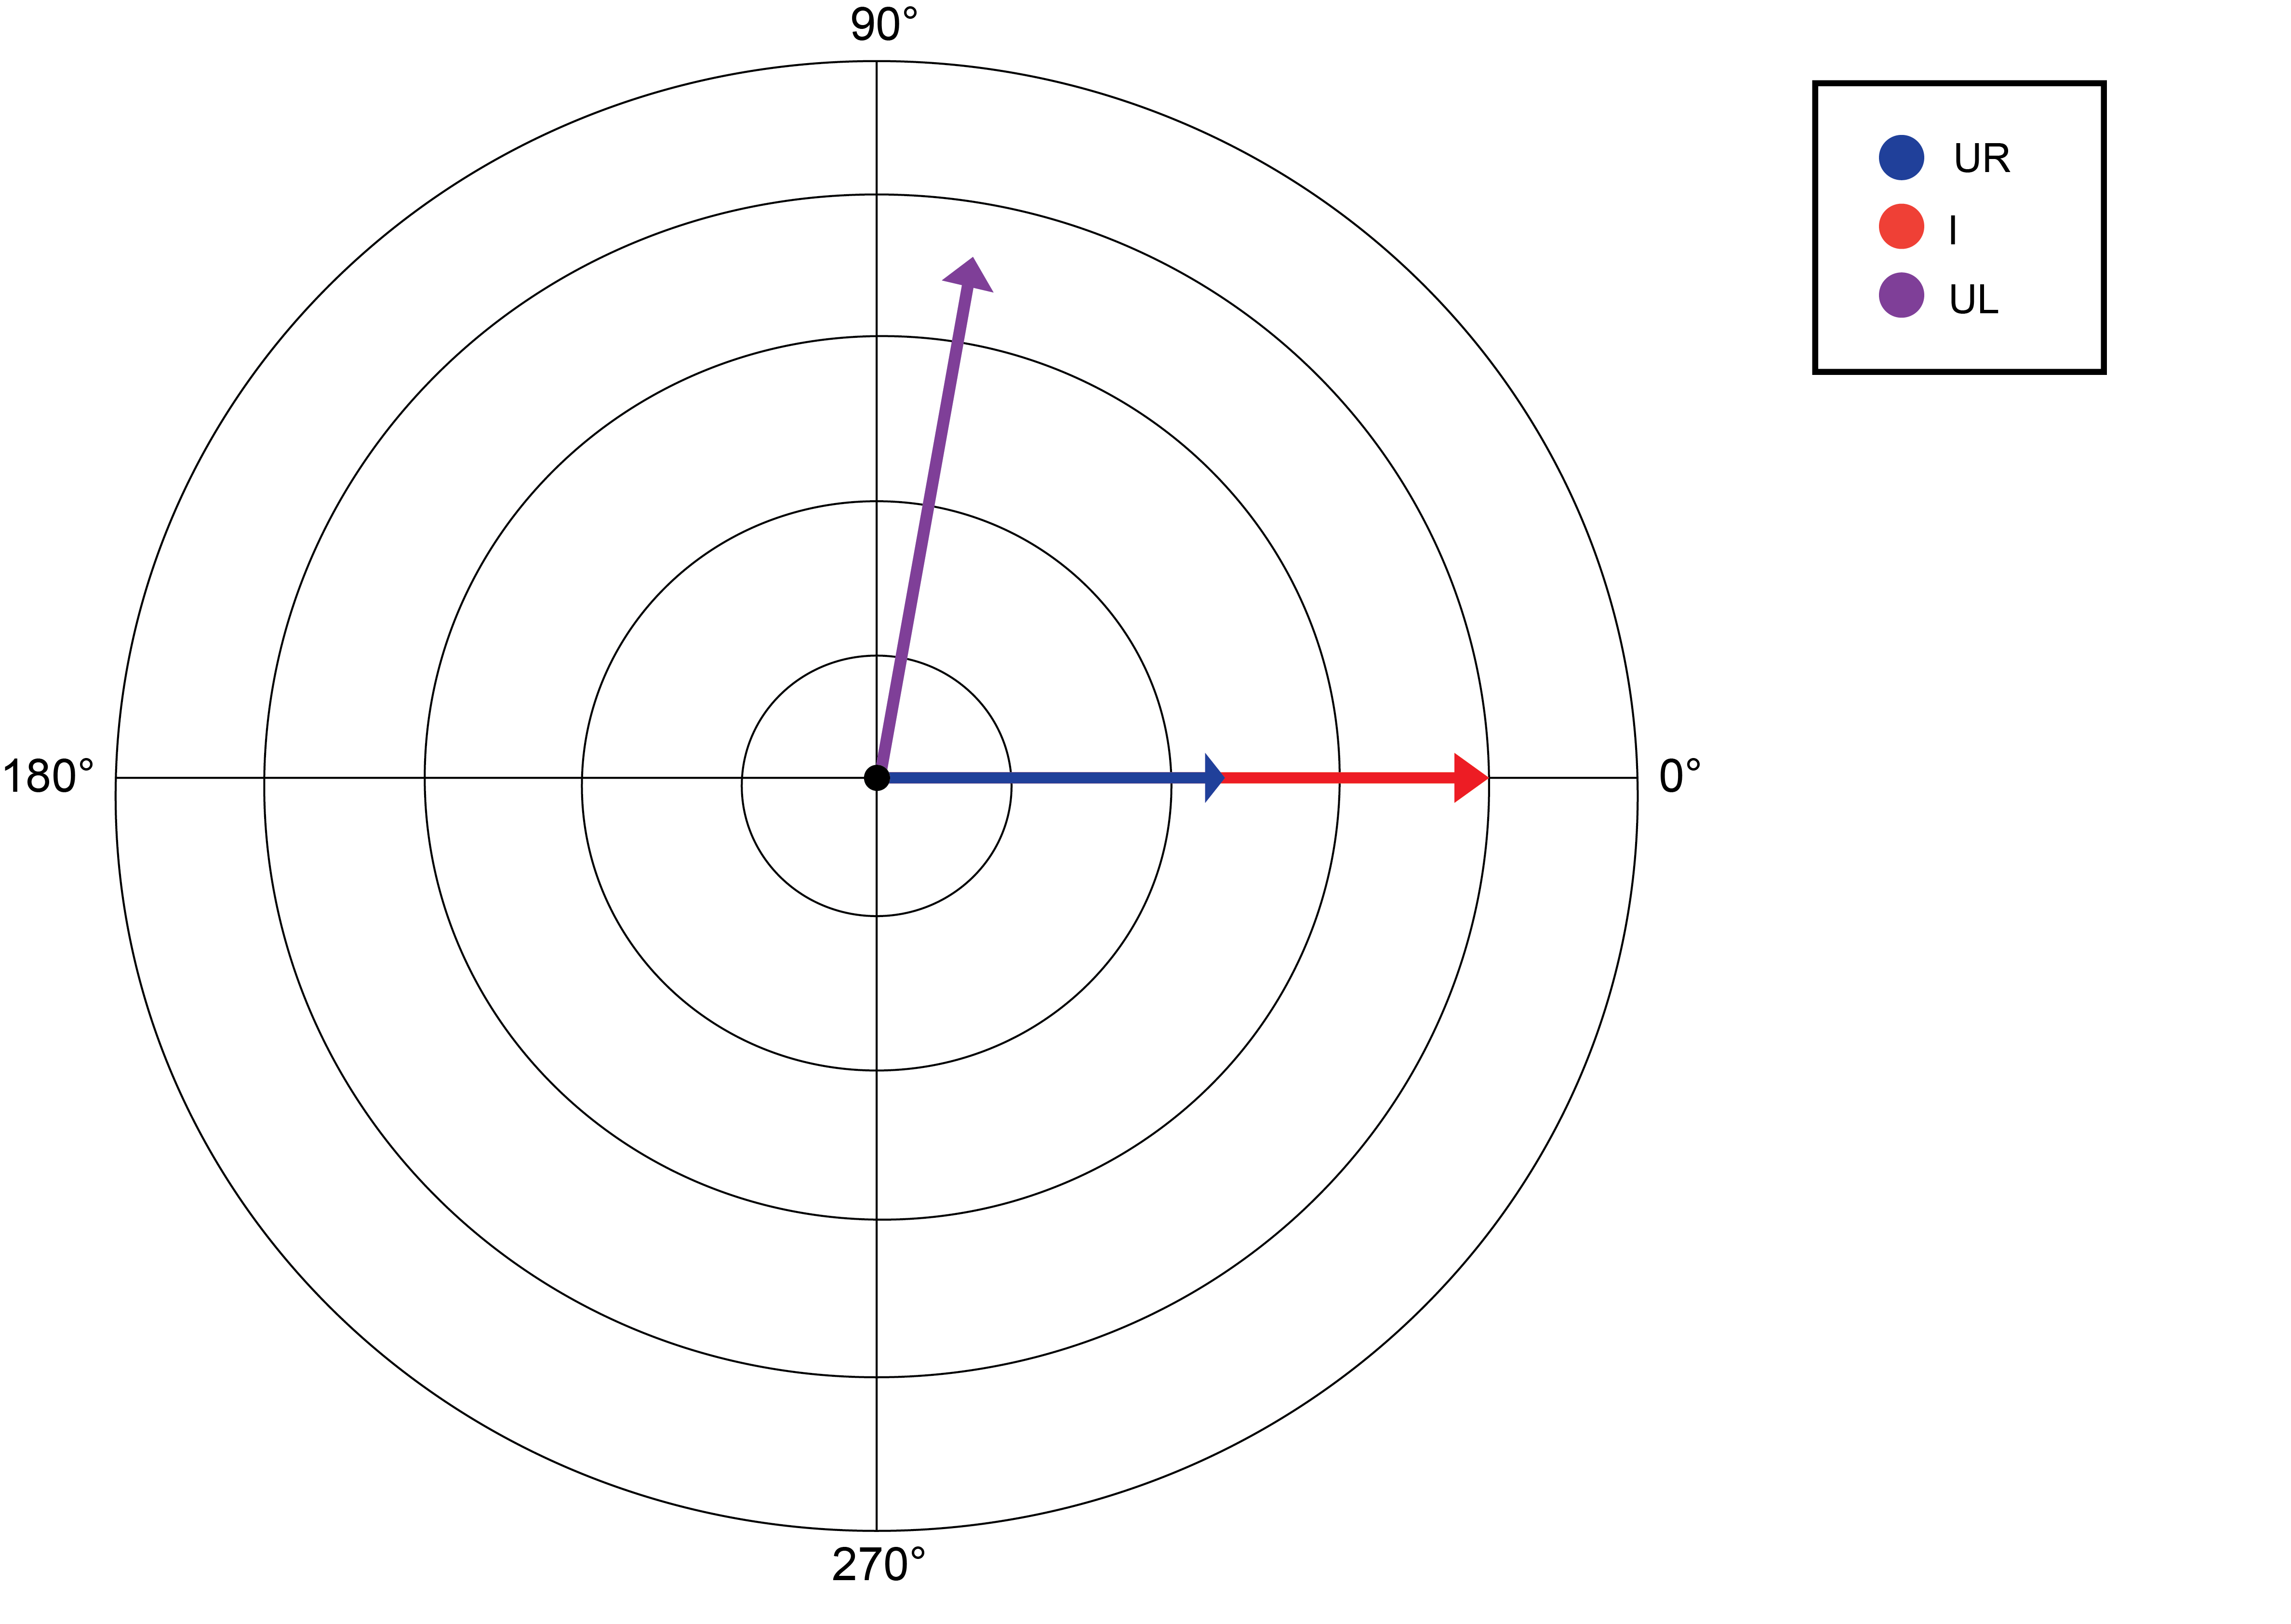
\includegraphics[width=0.6\linewidth]{nudes/Phasendiagramm4.png}
    \caption{Zeigerdiagramm der Phasenverschiebung der Spule}
    \label{fig:ZeigerdiagrammPhiL}
\end{figure}


\subsection{Elektrische Leistung RC-Schaltung}

Aus den Daten von Tabelle \ref{tab:Daten5} ergeben sich die Werte für $U$, $U_R$ und $U_C$. Die Phasenverschiebung $\phi_C$ ergibt sich aus dem zuvor berechneten Ergebnis aus Punkt Phasenlage Kondensator.

\begin{itemize}
    \item U = (13.0 $\pm$ 0.2) V
    \item $U_R$ = (9.09 $\pm$ 0.17) V
    \item $U_C$ = (8.86 $\pm$ 0.09) V
    \item $\phi_C$ = (-88.2 $\pm$ 0.3) °
\end{itemize}

\noindent
Mittels Formel \ref{eq:Phasenversatz_Kreise} kann nun der Phasenversatz zwischen Strom und und Eingangsspannung bestimmt werden.

\begin{itemize}
    \item $\phi$ = (-43.39 $\pm$ 0.13) °
\end{itemize}

\noindent
Aus den gewonnen Daten kann nun ebenfalls ein Zeigerdiagramm und ein Leistungsdreieck erstellt werden.

\begin{figure}[H]
    \centering
    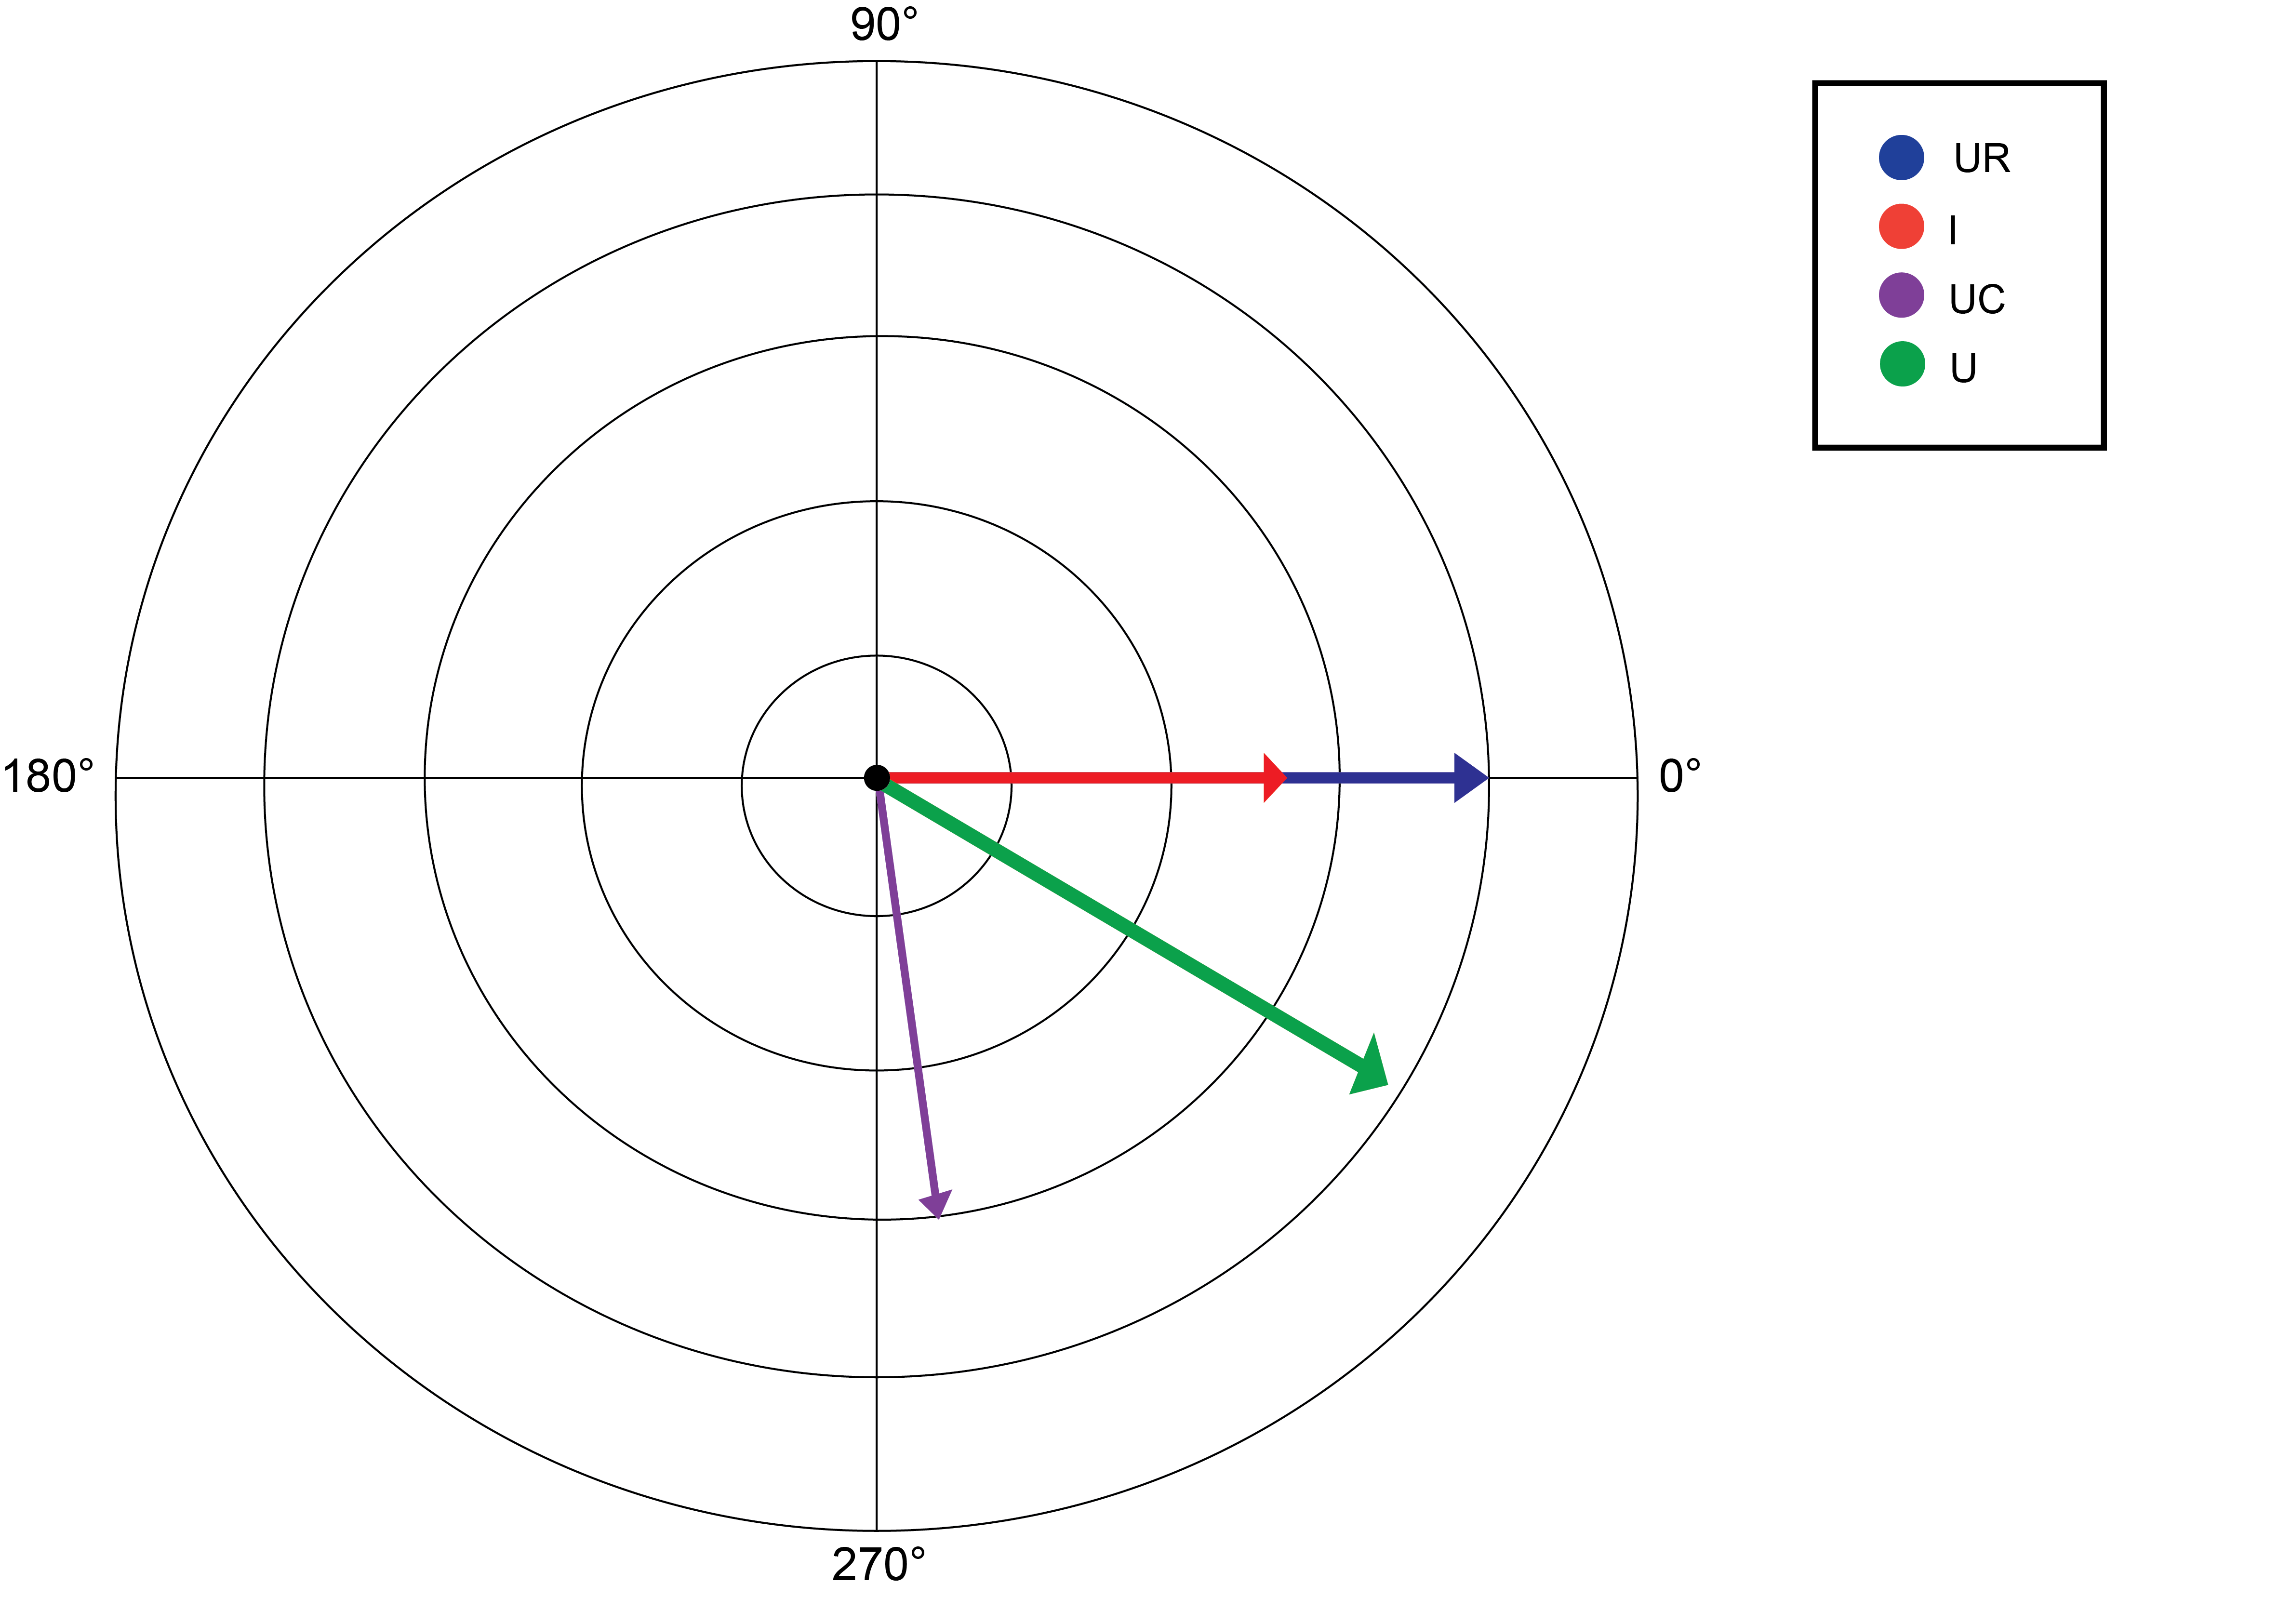
\includegraphics[width=0.6\linewidth]{nudes/Phasendiagramm5.png}
    \caption{Zeigerdiagramm RC-Kreis}
    \label{fig:ZeigerdiagrammRC}
\end{figure}

\begin{figure}[H]
    \centering
    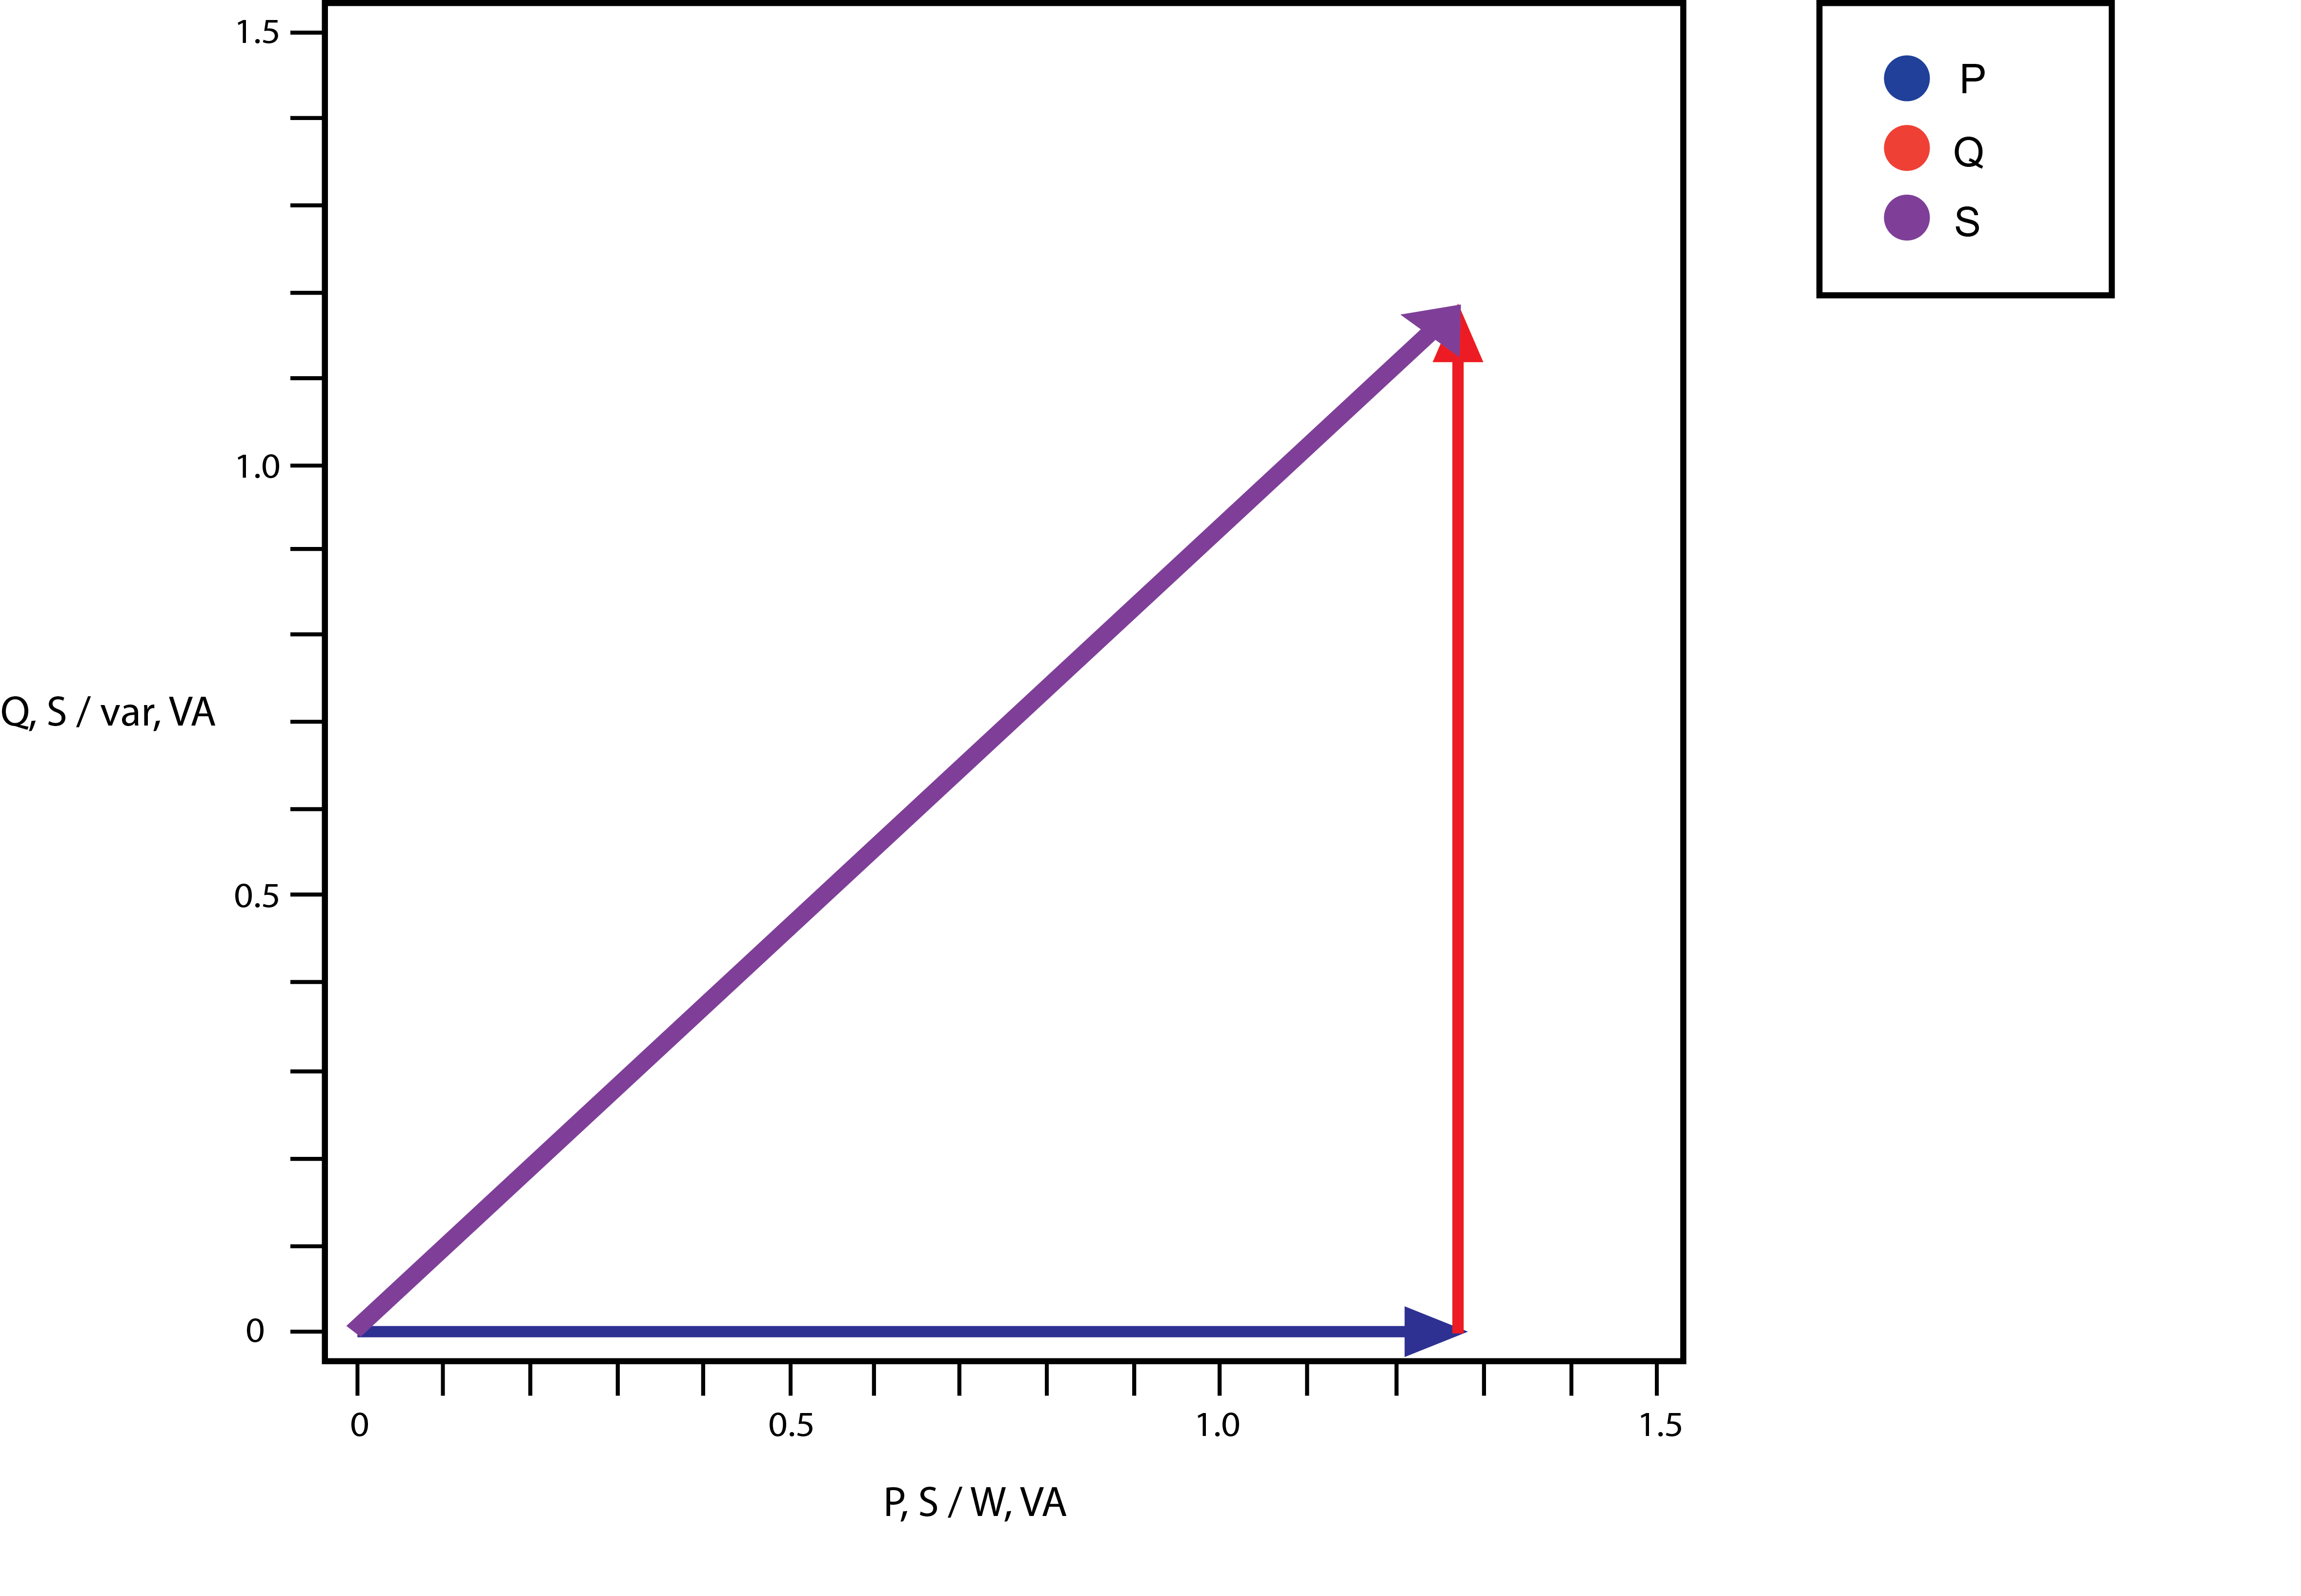
\includegraphics[width=0.6\linewidth]{nudes/Leistungsdreieck5.png}
    \caption{Leistungsdreieck RC-Kreis}
    \label{fig:LeistungsdreieckRC}
\end{figure}


\subsection{Elektrische Leistung RL-Schaltung}

Mit gleicher Vorgehensweiße wie in vorherigem Punkt lässt sich der Phasenversatz auch für die RL-Schaltung bestimmen. Aus Tabelle \ref{tab:Daten6} lassen sich wieder die benötigten Größen ablesen.

\begin{itemize}
    \item U = (13.6 $\pm$ 0.2) V
    \item $U_R$ = (3.35 $\pm$ 0.09) V
    \item $U_L$ = (12.82 $\pm$ 0.11) V
    \item $\phi_C$ = (84.6 $\pm$ 0.7) °
\end{itemize}

\noindent
Unter erneutem Verwenden von Formel \ref{eq:Phasenversatz_Kreise} lässt sich der neue Phasenversatz bestimmen.

\begin{itemize}
    \item $\phi$ = (70 $\pm$ 5) °
\end{itemize}

\noindent
Zu guter Letzt kann wieder ein Phasendiagramm und ein Leistungsdreieck gezeichnet werden.

\begin{figure}[H]
    \centering
    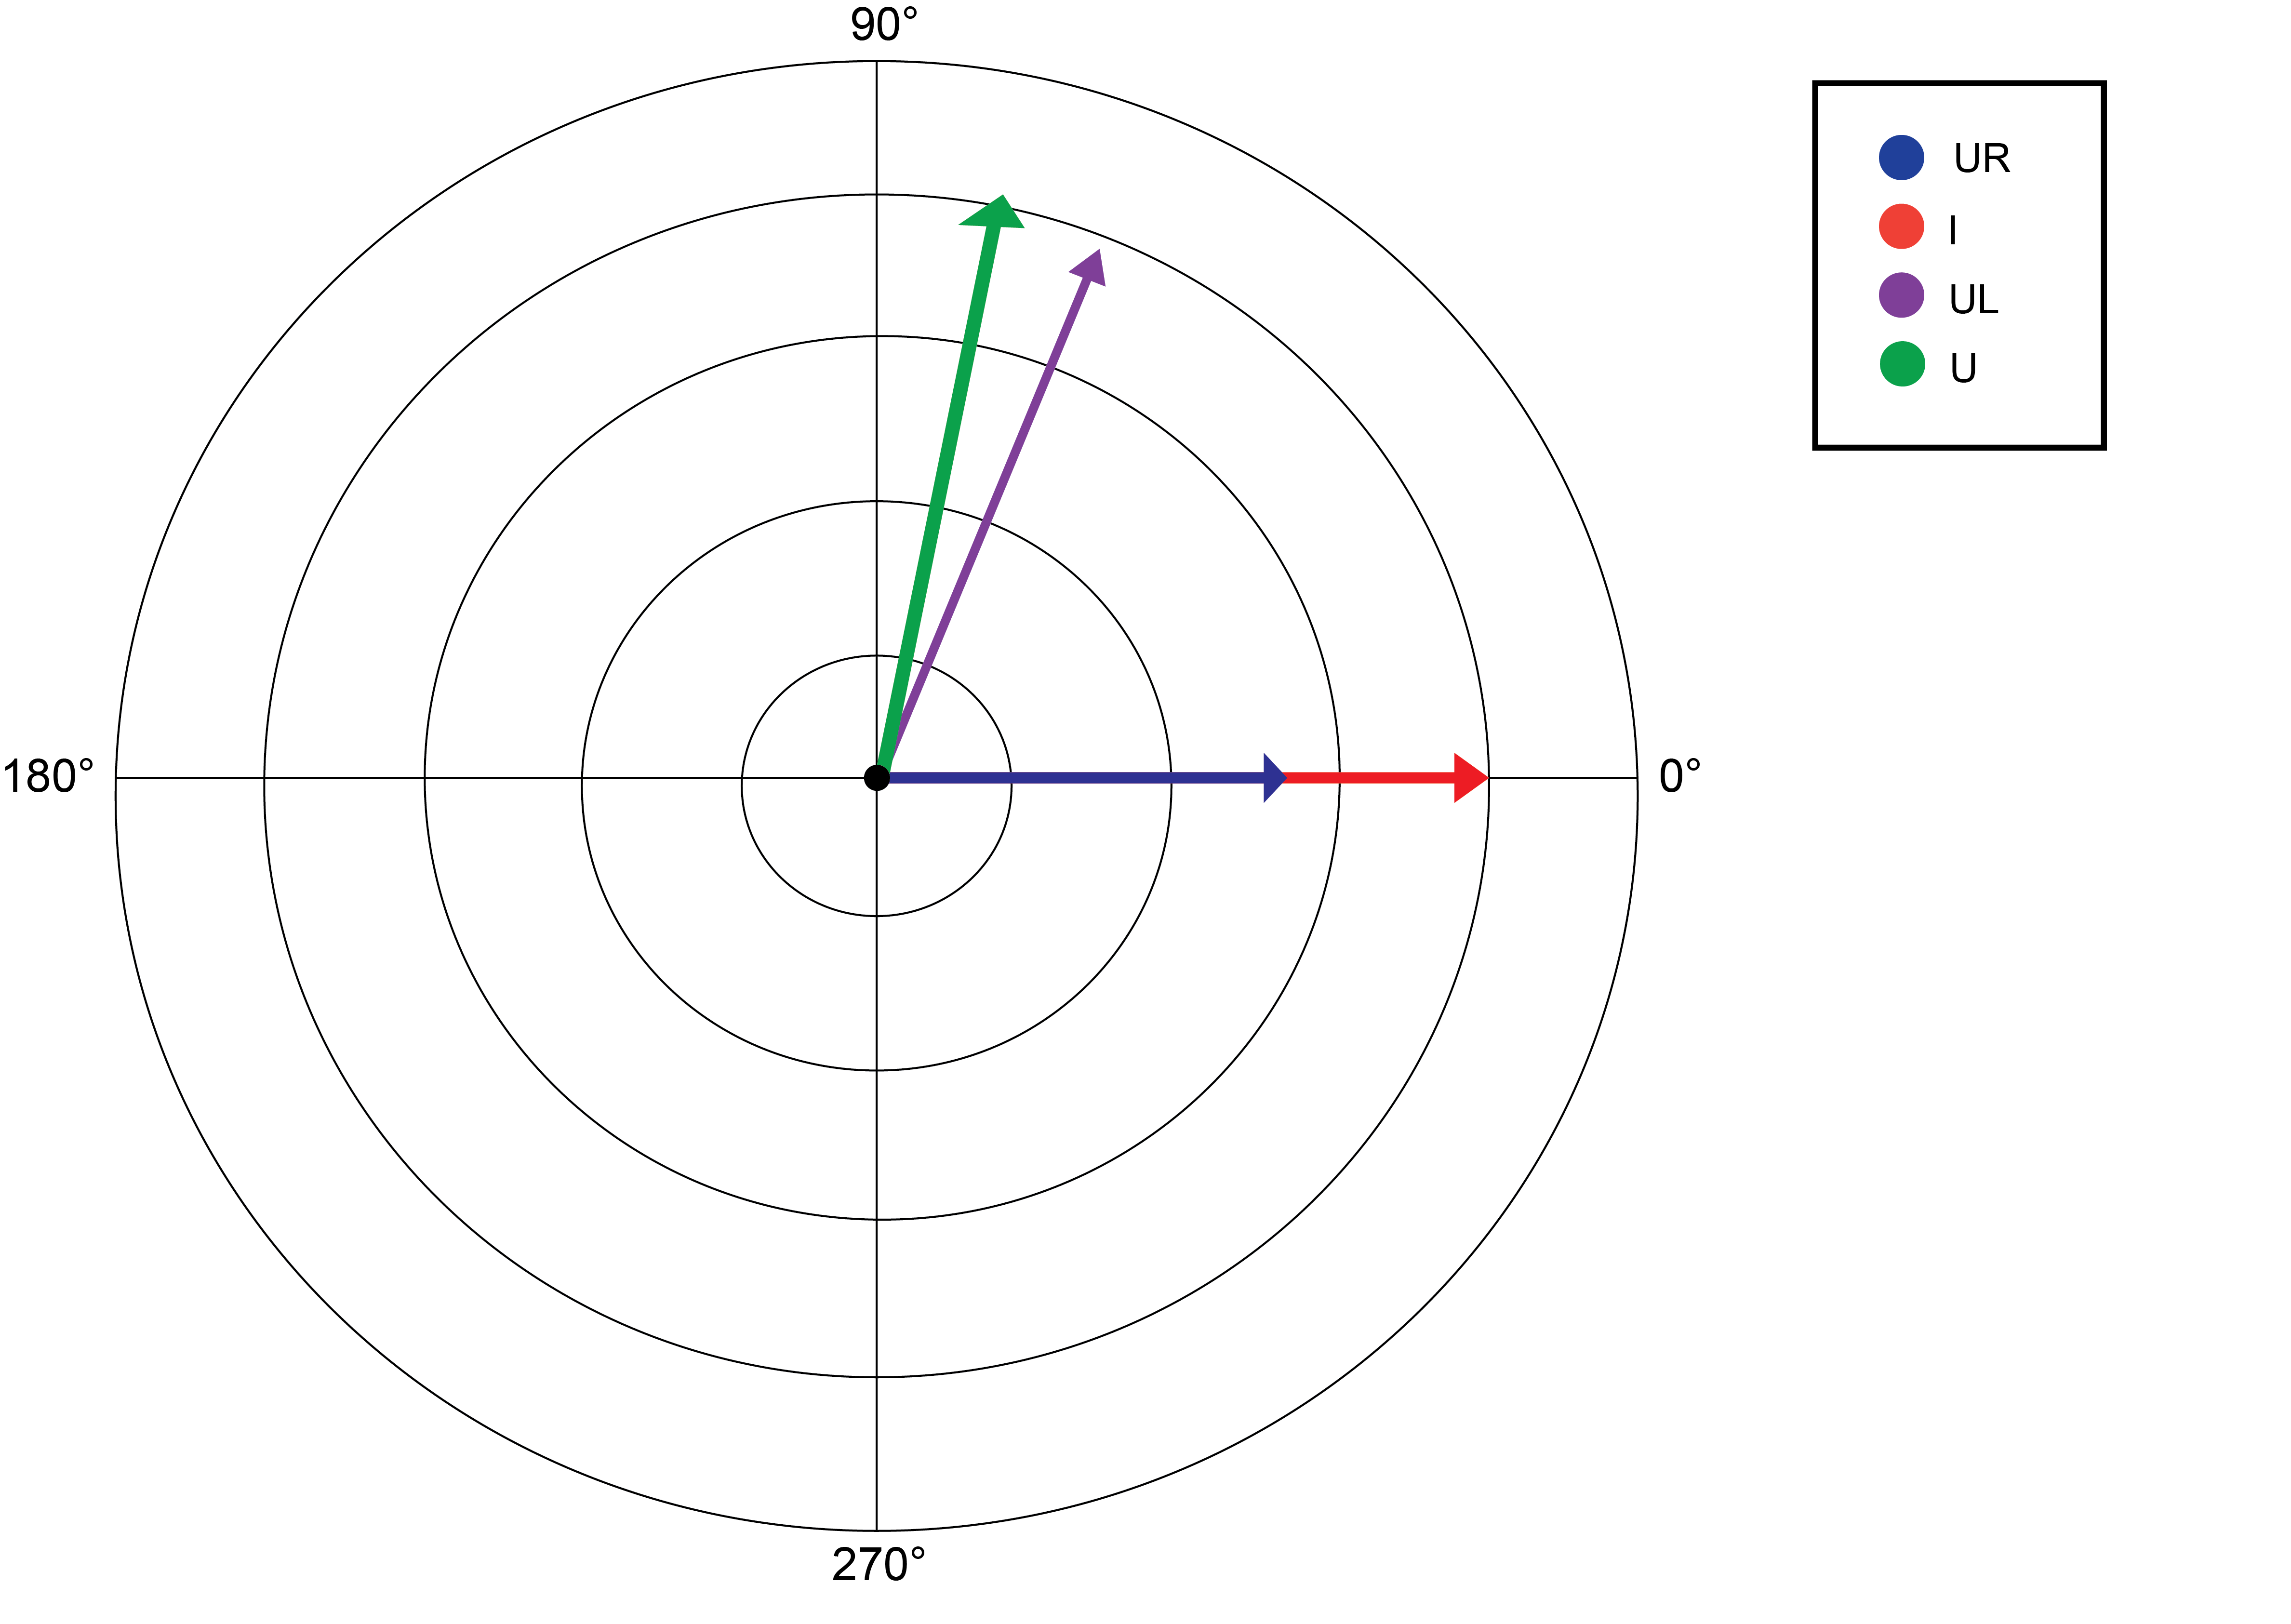
\includegraphics[width=0.6\linewidth]{nudes/Phasendiagramm6.png}
    \caption{Zeigerdiagramm RL-Kreis}
    \label{fig:ZeigerdiagrammRL}
\end{figure}

\begin{figure}[H]
    \centering
    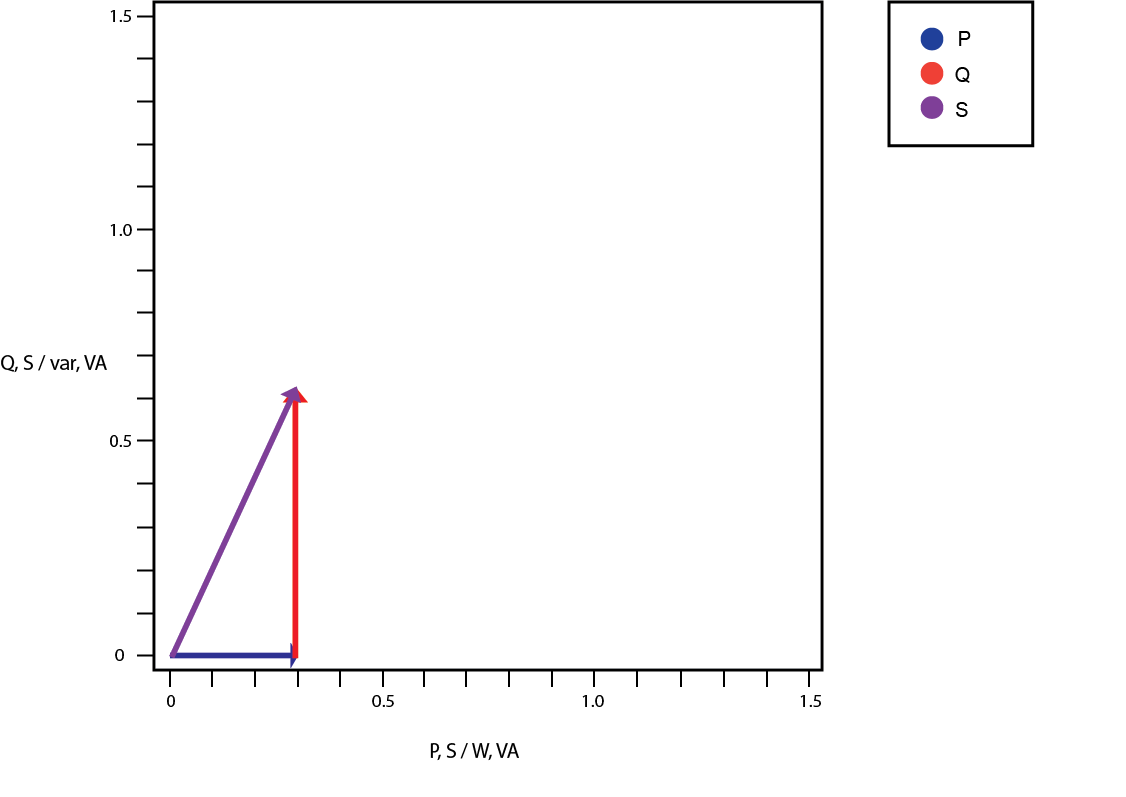
\includegraphics[width=0.6\linewidth]{nudes/Leistungsdreieck6.png}
    \caption{Leistungsdreieck RL-Kreis}
    \label{fig:LeistungsdreieckRL}
\end{figure}


\subsection{Blindleistungskompensation}

Aus der verwendeten Induktivität von L = 1H und der verwendeten Kapazität C = 47 $\mu F$ ergeben sich unter Verwendung der Formeln \ref{eq:ReaktanzenC} und \ref{eq:ReaktanzenL} die Reaktanzen $X_C$ und $C_L$.

\begin{itemize}
    \item $X_C$ = (68 $\pm$ 3) $\Omega$
    \item $X_L$ = (314 $\pm$ 15) $\Omega$
\end{itemize}

\noindent
Aus den Reaktanzen ergeben sich mit den Verlusten $R_C$/$R_L$ die komplexen Impedanzen $Z_C$/$Z_L$:

\begin{equation}
    \label{eq:ImpedanzC}
    \centerline{$Z_{C}$ = $\frac{(X_C)^2}{R_C}$ \\ $\Delta Z_{C} = \vert \frac{\partial Z_{C}}{\partial X_C} * \Delta X_C \vert + \vert \frac{\partial Z_{C}}{\partial R_C} * \Delta R_C \vert $ } 
\end{equation}

\begin{equation}
    \label{eq:ImpedanzL}
    \centerline{$Z_{L}$ = $R_L + X_L$ \\ $\Delta Z_{L} = \vert \frac{\partial Z_{L}}{\partial X_L} * \Delta X_L \vert + \vert \frac{\partial Z_L}{\partial R_L} * \Delta R_L \vert $ }
\end{equation}

\begin{itemize}
    \item $Z_C$ = (68 $\pm$ 3) $\Omega$
    \item $Z_L$ = (315 $\pm$ 14) $\Omega$
\end{itemize}

\noindent
Die dazugehörigen Phasenversätze ergeben sich dabei mit:

\begin{equation}
    \label{eq:PhvZL}
    \centerline{$\phi_L = arctan(\frac{-X_L}{R_L})$ \\ $\Delta Z_{L} = \vert \frac{\partial Z_{L}}{\partial X_L} * \Delta X_L \vert + \vert \frac{\partial Z_{L}}{\partial R_L} * \Delta R_L \vert $ }
\end{equation}

\begin{equation}
    \label{eq:PhvZC}
    \centerline{$\phi_C = arctan(\frac{-X_C}{R_C})$ \\ $\Delta Z_{C} = \vert \frac{\partial Z_{C}}{\partial X_C} * \Delta X_C \vert + \vert \frac{\partial Z_{C}}{\partial R_C} * \Delta R_C \vert $ }
\end{equation}

\begin{itemize}
    \item $\phi_{Z_L}$ = (-87.17 $\pm$ 0.41) °
    \item $\phi_{Z_C}$ = (77.11 $\pm$ 0.34) °
\end{itemize}

\noindent
Abschließend können nun die geforderten Phasenversätze mittels folgenden Formeln bestimmt werden.

\begin{equation}
    \label{eq:PhvU}
    \centerline{$\phi_U = arg(Z_C \left\lvert\right\rvert Z_L)$ }
\end{equation}

\begin{equation}
    \label{eq:PhvL/C}
    \centerline{$\phi_{L/C} = arg(Z_C \left\lvert\right\rvert Z_L)$ }
\end{equation}

\begin{itemize}
    \item $\phi_U$ = (22 $\pm$ 4) °
    \item $\phi_L/C$ = (20 $\pm$ 4) °
\end{itemize}

\noindent
Mittels Formeln \ref{eq:Scheinleistung} - \ref{eq:Blindleistung} können nun die Werte für Schein-, Blind- und Wirkleistung bestimmt werden.

\begin{itemize}
    \item S = (1.49 $\pm$ 0.26) VA
    \item Q = (-0.56 $\pm$ 0.08) var
    \item P = (1.38 $\pm$ 0.21) W
\end{itemize}

\noindent
Somit lassen sich auch ein weiteres Zeigerdiagramm und Leistungsdreieck erstellen.

\begin{figure}[H]
    \centering
    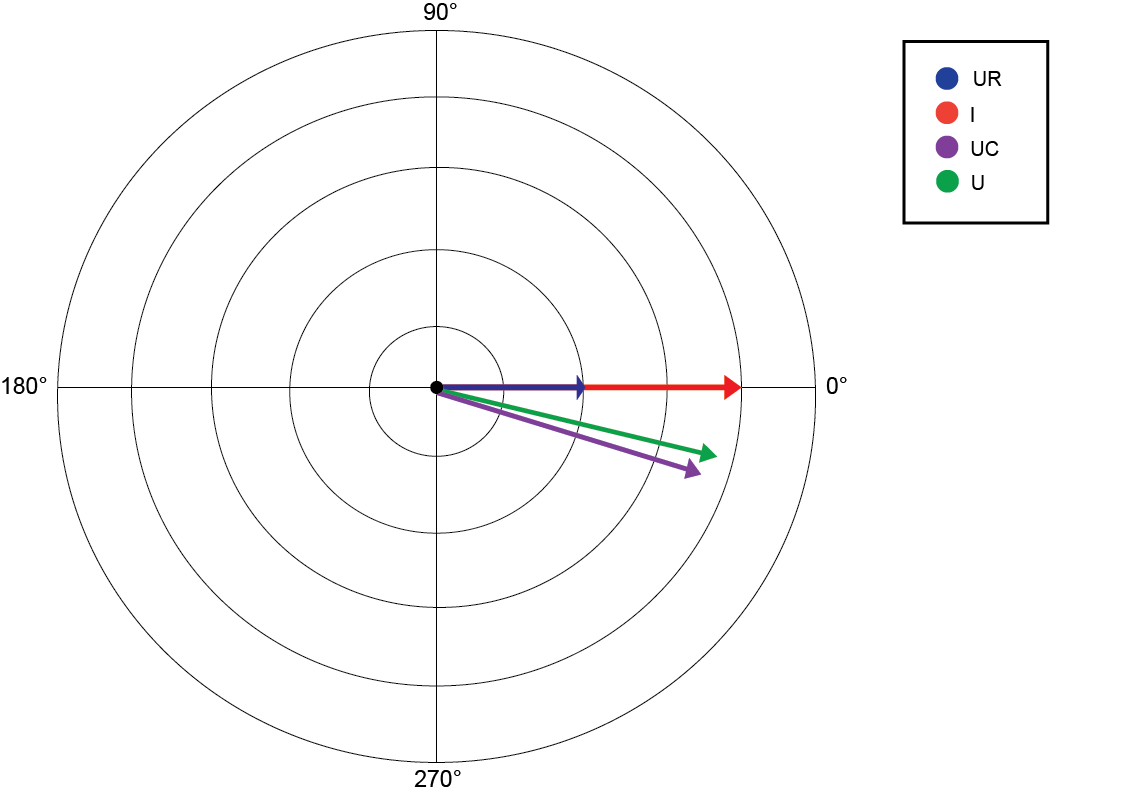
\includegraphics[width=0.6\linewidth]{nudes/Phasendiagramm7.png}
    \caption{Zeigerdiagramm RLC-Kreis}
    \label{fig:ZeigerdiagrammRLC}
\end{figure}

\begin{figure}[H]
    \centering
    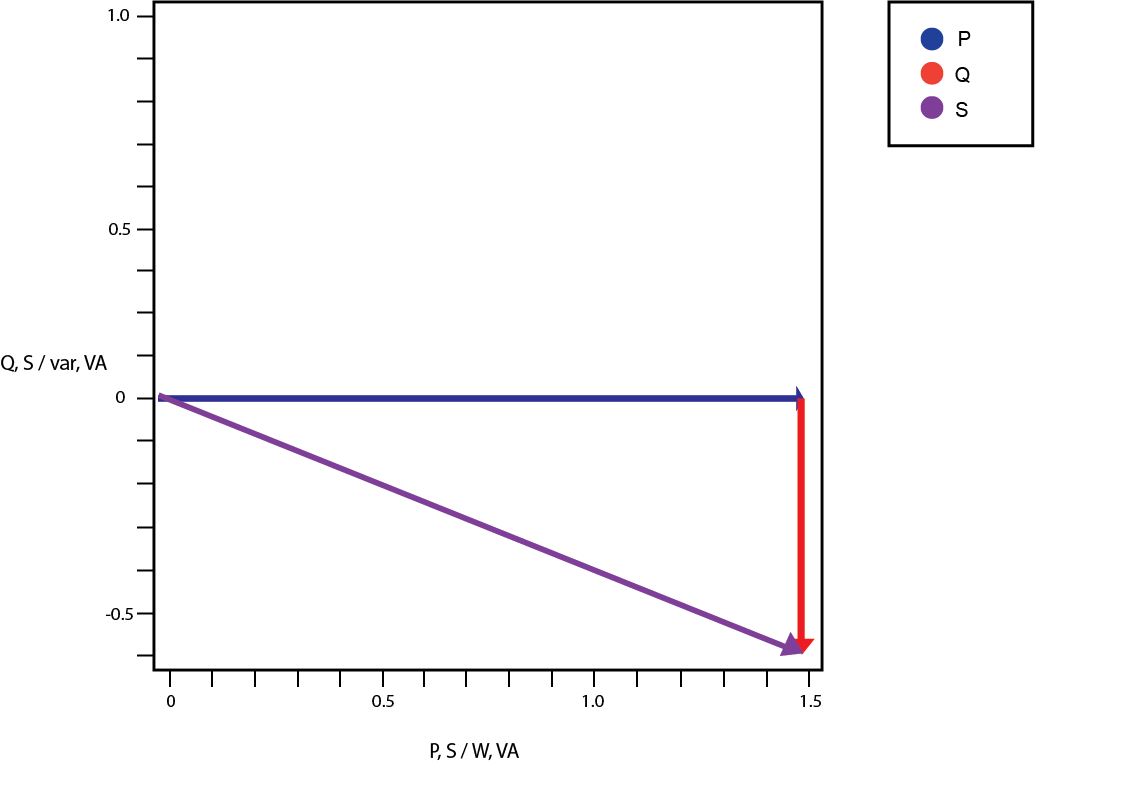
\includegraphics[width=0.6\linewidth]{nudes/Leistungsdreieck7.png}
    \caption{Leistungsdreieck RLC-Kreis}
    \label{fig:LeistungsdreieckRLC}
\end{figure}


\section{Diskussion} %diskussion der Unsicherheiten und Ergebnisse und evtl. verlgeich mit Literatur ------------------------------

\subsection{Untersuchung der Anzeigen / Amplitudengänge}

Den Resultaten der ersten Aufgabe ist zu entnehmen, dass es für verschiedene Geräte einen Unterschied macht, mit welchem Signal und welcher Frequenz gearbeitet wird.
Somit ist darauf zu achten, um fehlerhafte Messergebnisse zu vermeiden.


\subsection{Phasenlage Kondensator / Spule}

Die resultierenden Zeigerdiagramme zeigen die Wirkung der Kapazität und Induktivität als Reaktanzen. 
Aufgrund von Innenwiderständen haben aber auch sie einen Einfluss auf die reale Leistung der Schaltung und müssen miteinbezogen werden.
Es lässt sich außerdem erkennen, dass bei der Kapazität die Spannung dem Strom "hinterherhengt", und bei Induktivität die Spannung dem Strom "vorauseilt".

\subsection{Elektrische Leistung RC-Schaltung / RL-Schaltung}

Anhand der resultierenden Blindleistung, welche in den vorherigen Teilen bestimmt wurde, lässt sich erkennen, dass die Leistung nicht nur vom ohm`schen Widerstand, sondern auch von inneren Widerständen der Kapazität/Induktivität abhängt.

\subsection{Blindleistungskompensation}

Die Blindleistungskompensation wurde bestmöglich zu bestimmen versucht.  


\section{Zusammenfassung} %klare, übersichtliche vollständige beantwortung der Aufgabenstellung ------------------------------

\subsection{Untersuchung der Anzeigen}

Das Problem wurde im Punkt Auswertung diskutiert.


\subsection{Amplitudengänge}

Die Amplitudengänge sind in Abbildung \ref{fig:Amplitudengänge} ersichtlich.


\subsection{Phasenlage Kondensator}

$\phi_C$ = (-88.2 $\pm$ 0.3) ° 


\subsection{Phasenlage Spule}

$\phi_L$ = (84.6 $\pm$ 0.7) ° 


\subsection{Elektrische Leistung RC-Schaltung}

Zeigerdiagramm und Leistungsdreieck wurden, ersichtlich in den Abbildungen \ref{fig:ZeigerdiagrammRC} und \ref{fig:LeistungsdreieckRC}, ermittelt.

\subsection{Elektrische Leistung RL-Schaltung}

Zeigerdiagramm und Leistungsdreieck wurden, ersichtlich in den Abbildungen \ref{fig:ZeigerdiagrammRL} und \ref{fig:LeistungsdreieckRL}, ermittelt.

\subsection{Blindleistungskompensation}

Zeigerdiagramm und Leistungsdreieck wurden, ersichtlich in den Abbildungen \ref{fig:ZeigerdiagrammRLC} und \ref{fig:LeistungsdreieckRLC}, ermittelt.


\printbibliography[heading=bibintoc]
\end{document}
